% This is LLNCS.DOC the documentation file of
% the LaTeX2e class from Springer-Verlag
% for Lecture Notes in Computer Science, version 2.4
\documentclass{llncs}
\usepackage{llncsdoc}

%
\usepackage[dvipdfmx]{graphicx}
\usepackage{subfigure}
\usepackage{bm}
\usepackage{amsmath}
\def\vect#1{\mbox{\boldmath$#1$}}

\begin{document}

\title{Anthropomorphic Finger Mechanism with a non-elastic Branching Tendon}
\author{Kazuya Yanagisawa, Shouhei Shirafuji, Shuhei Ikemoto, Koh Hosoda
\thanks{This work was supported by JSPS KAKENHI Grant Numbers 23650098, 24-3541.}}
\institute{Information Science and Technology, Osaka University \email{yanagisawa.kazuya@ist.osaka-u.ac.jp}}
\maketitle

\begin{abstract}
	To realize both grasp
	stability and manipulation dexterity is a central
	problem in teh development of robot hands.
	% ロボットハンドにとってもっとも重要なのは,物体の安定把持と細かな操作を
	% 両立することである.
	In recent years, many underactuated robot hands have been developed that
	flexibly conform to an object's surface with %a 
	simple control.
	% system.
	% 近年,関節の数よりも少ないアクチュエータで駆動する劣駆動ハンドが多く開
	% 発され,一般的なロボットハンドに比べて簡単な制御で,物体表面に適応する
	% 柔らかな物体把持が実現されている.
	
	In contrast, it is difficult to realize dexterous manipulation 
	by such underactuated hands in which
	%requires to control 
	all degrees of freedom (DoFs) should be controlled.
	% しかし,劣駆動ハンドの場合には,アクチュエータの少なさから,細かな操作
	% を実現するのは難しい.
	In this research, to realize the dexterous manipulation
	by simple mechanism and control,
	we develop a robot gripper comprising of two tendon-driven robotic fingers
	with non-elastic branching tendons.
	% In this research, we develop a robot gripper consists of two
	% tendon-driven robotic fingers with non-elastic branching tendons to
	% overcome the problem to realize dexterous manipulation by simple
	% mechanism and control.
	% 本論文では,劣駆動のような簡易な制御で,細かい操作を実現するために,非
	% 伸縮な分岐腱をもつロボットフィンガで構成されたグリッパを開発することを
	% 目的とする.
	The branching tendon is a tendon that branches out and connects an actuator
	to different links.
	% The branching tendon indicates a tendon which branches and connect an
	% actuator to different links.
	% 分岐腱とは,1つのアクチュエータにつながれた腱が,ある点で複数の腱に分岐
	% したものである.
	% In particular, we focus on the non-elastic branching tendon that
	% connects an actuator to links of two DoFs robotic finger.
	% ここでは,分岐腱構造としてもっとも単純な,2関節2腱のロボットフィンガを
	% 考える.
	The two joints of this robotic finger are coupled by the non-elastic
	branching tendon when no external force is exerted.
	% In this robotic finger, the displacement angles of the two joins are
	% coupled by the non-elastic branching tendon in the situation where no
	% external force is exerted.
	% 分岐腱が非伸縮な場合,フィンガは,外力がない状態では,幾何学的な拘束に
	% より関節が連動して1自由度で動作する.
	If sufficient external force is applied to the fingertip,
	one of the tendons slackens and the coupling between the two joints is lost.
	% If a certain amount of external force is applied on the fingertip, the
	% branching tendon can be slack and the coupling between two joints is
	% broken.
	% 一方,フィンガの出す力や物体からの拘束といった条件によっては,分岐腱に
	% 緩みが生じ,関節の連動が生じなくなる.
	This means that the two-DoF robotic finger is easily controlled as a single
	DoF mechanism when reaching toward an object, but when the fingertip is placed on the object,
	the coupling provided by the branching tendon is released and the finger shifts.
	% つまり,物体に接触するまでは,1自由度として簡易な制御で動作させることが
	% でき,指先が拘束されても,分岐腱を緩ませて関節の連動をなくすことでフィ
	% ンガの姿勢と指先位置を変化させ,把持後の物体操作を実現できる.
	Based on this idea, we develop and control a two-DoF robotic finger
	equipoed with two tendons including a non-elastic branching tendon.
	% 以上をふまえ,2関節2腱のロボットフィンガを開発し,その制御を行った.
	We also analyse the conditions, where the branching tendon slacken, and confirmed in an experiment. 
	% さらに,分岐腱に緩みが生じるための力学的条件を考察し,実機で検証した.
	As the result, the availability of controlling the slack of branched
	tendon was successfully confirmed.
	% その結果,意図的に分岐腱を緩ませる,もしくは緩ませないような制御ができ
	% ることを示した.
\end{abstract}

% \markboth{\LaTeXe{} Class for Lecture Notes in Computer
% Science}{\LaTeXe{} Class for Lecture Notes in Computer Science}
% \thispagestyle{empty}
% \begin{flushleft}
% \LARGE\bfseries Instructions for Authors\\
% Coding with \LaTeX\\[2cm]
% \end{flushleft}
% \rule{\textwidth}{1pt}
% \vspace{2pt}
% \begin{flushright}
% \Huge
% \begin{tabular}{@{}l}
% \LaTeXe{} Class\\
% for Lecture Notes\\
% in Computer Science\\[6pt]
% {\Large Version 2.4}
% \end{tabular}
% \end{flushright}
% \rule{\textwidth}{1pt}
% \vfill
% %\begin{flushleft}
% %\large\itshape
% %\begin{tabular}{@{}l}
% %{\Large\upshape\bfseries Springer}\\[8pt]
% %Berlin\enspace Heidelberg\enspace New\kern0.1em York\\[5pt]
% %Barcelona\enspace Budapest\enspace Hong\kern0.2em Kong\\[5pt]
% %London\enspace Milan\enspace Paris\enspace\\[5pt]
% %Santa\kern0.2em Clara\enspace Singapore\enspace Tokyo
% %\end{tabular}
% %\end{flushleft}
% \newpage
% %
% \section*{For further information please contact us:}
% %
% \begin{flushleft}
% \begin{tabular}{l@{\quad}l@{\hspace{3mm}}l@{\qquad}l}
% $\bullet$&\multicolumn{3}{@{}l}{\bfseries LNCS Editorial Office}\\[1mm]
% &\multicolumn{3}{@{}l}{Springer-Verlag}\\
% &\multicolumn{3}{@{}l}{Computer Science Editorial}\\
% &\multicolumn{3}{@{}l}{Tiergartenstra゚e 17}\\
% &\multicolumn{3}{@{}l}{69121 Heidelberg}\\
% &\multicolumn{3}{@{}l}{Germany}\\[0.5mm]
%  & Tel:       & +49-6221-487-8706\\
%  & Fax:       & +49-6221-487-8588\\
%  & e-mail:    & \tt lncs@springer.com    & for editorial questions\\
%  &            & \tt texhelp@springer.de & for \TeX{} problems\\[2mm]
% \noalign{\rule{\textwidth}{1pt}}
% \noalign{\vskip2mm}
% %
% %{\tt svserv@vax.ntp.springer.de}\hfil first try the \verb|help|
% %command.
% %
% $\bullet$&\multicolumn{3}{@{}l}{\bfseries We are also reachable through the world wide web:}\\[1mm]
%          &\multicolumn{2}{@{}l}{\texttt{http://www.springer.com}}&Springer Global Website\\
%          &\multicolumn{2}{@{}l}{\texttt{http://www.springer.com/lncs}}&LNCS home page\\
%          &\multicolumn{2}{@{}l}{\texttt{http://www.springerlink.com}}&data repository\\
%          &\multicolumn{2}{@{}l}{\texttt{ftp://ftp.springer.de}}&FTP server
% \end{tabular}
% \end{flushleft}


% %
% \newpage
% \tableofcontents
% \newpage
%

\section{Introduction} % (fold)
\label{sec:introduction}
Humanlike stability and dexterous object manipulation has been a central focus in robotic hand research.
% ロボットのエンドエフェクタ,特にロボットハンドの開発における目標の一つと
% して,ヒトの手のような物体の安定把持と細かな操作の両立があげられる.
% During object manipulation, because a robot's body has to be controlled
% at the same time as the control of the hand, to simplify the control to
% reduce consumption of compuational resource is important.
% さらに,ロボットに実装する場合,ロボットの全身を同時に制御する必要からハ
% ンドに割ける計算能力には限界があるため,より簡便な制御でこれを実現するこ
% とも重要である.
The hardware of robot hands is designed in two ways;
by actuating joints directly by motors and by actuating joints through tendons.
% ロボットハンドの駆動方式としては,関節を直接モータなどで駆動する方式と,
% 腱により駆動する方式がある.
When a robot hand is designed to imitate a compact human's hand,
a tendon-driven mechanism is often employed
since it does not necessarily put motors at the joints.
% 小型で,特にヒトを規範とするロボットハンドにおいては,関節にモータを組み
% 込むことの空間的な制約があること,また,ヒトの手を模倣するという観点から,
% 腱駆動を採用することがまず考えられる.
Examples of tendon-robotic hands are JPL/Stanford Hand\cite{salisbury1982}, Utah/MIT
Hand\cite{Jacobsen1986},and DLR-Hand\cite{Butterfass2001} are all
employing the tendon-driven mechanism.
% 腱駆動のロボットハンドとしては,JPL/Stanford Hand\cite{Loucks1987}や,
% Utah/MIT Hand\cite{Jacobsen1986},DLR-Hand\cite{Butterfass2001}などが有
% 名である.
In particular, ACT Hand\cite{vande2004} has very similar musculotendinous
structure to a human hand.
% また,ヒトの手の構造を模倣したロボットハンドに,ACT Hand\cite{Weghe2004}
% がある.
A sufficient versatile dexterous robot hand requires many degrees of freedom(DoFs).
% Generally speaking, when we try to design a dexterous robot hand,
% we tend to put many degrees of freedom (DoFs) to the hand
% so that we can make it more versatile.
% 一般に,物体の細かな操作を実現するためには,多くの自由度をもったロボット
% ハンドが必要になる.
To achieve such versatility, the system must control more tendons than joints;
that is, it must control the number of DoFs.
% However in order for these tendon-driven hands to this end,
% tendons more than the number of joints (i.e. the number of DoFs) have to be controlled.
% しかし,これらのロボットハンドのように腱駆動方式で制御するためには,関節
% の数,つまり自由度よりも多くの腱が必要になる.
As the number of DoFs increases, controlling becomes increasingly complex.
% Therefore, control becomes complex and difficult as the number of DoFs increases.
% そのため,自由度を保ったままハンドを駆動しようとすると,関節を直接駆動す
% る場合に比べてアクチュエータの数が増加してしまい,制御が複雑になるという
% 問題がある.

% To overcome this problem, in recent years, an approach to decrease
% complexity of control by designing a hardware which can bear a part of
% computaion in the control\cite{Pfeifer2010}.
% % この制御の複雑さという問題に対して,近年,制御の一部をロボットの機構や形
% % 態,もしくはシステムと環境との相互作用の中に取り込むことで制御の計算量を
% % 減らす方法が考えられている\cite{Pfeifer2010}.
% % 実環境で用いられるロボットは,常に環境からの影響を受けて動作している.
% % したがって,すべてを制御して目的の振る舞いをさせようとするのではなく,環
% % 境と相互作用することで目的の振る舞いをするような機構が注目されている.

To overcome this problem, a hand which has less actuators,
which is called an underactuated mechanism, has been researched\cite{Birglen2008}.
% このような形態への制御の取り込みとして,関節の数よりも少ないアクチュエー
% タでロボットを駆動する,劣駆動についての研究が進められている
% \cite{Birglen2008}.
For example, Soft Gripper, which realixes flexible encapsulation grasping\cite{Hirose1978}
and 100G Hand, which accomplishesa fast catching task\cite{Kaneko2003}
% For instance, Soft Gripper realized flexible encapsulation
% grasping\cite{Hirose1978} and 100G Hand accomplished fast catching
% task\cite{Kaneko2003}.
% 劣駆動のロボットハンドとしては,柔らかな包み込み把持を実現したSoft
% Gripper\cite{Hirose1978}を始めとし,高速なキャッチングが可能な100G
% Hand\cite{Kaneko2003}などがある.
These hands can be simplified because they replace actuators with passive mechanical elements
such as springs.
% These hands can be simplified since they employ passive mechanical elements
% such as springs instead of actuators.
% これらのハンドでは,一部のアクチュエータの代わりにバネのような受動素子を
% 組み合わせることでアクチュエータの数を減らし,構造,制御を簡略化してい
% る.
% さらに,受動素子を取り入れることで物体と接触したときには柔らかい把持を行
% えるように設計されている.
TUAT/Karlsruhe Hand has five underactuated fingers comprising rigid linkages
and is capable to realize various types of grasping\cite{Fukaya2013}.
% また,TUAT/Karlsruhe Hand\cite{Fukaya2013}では,ロッドの組み合わせにより
% 5指の劣駆動を行い,さまざまな姿勢の物体把持を実現している.
% However, on account of their low DoFs, underactuated hands are
However, an underactuated hand is often designed to be specialized for specific tasks
because it basically has less DoFs.
% しかし,劣駆動ハンドは,アクチュエータの少なさから,特定の機能を目的とし
% て設計することが多く,さまざまなタスクをこなせるハンドにはなりにくい.
% また,受動素子のおかげで柔らかい物体把持を可能にする一方で,指先の細かな
% 位置制御などは難しくなり,物体をハンドの中で操作すると行った細かい動作を
% 実現している例は少ない.

In real human hands, the distal extensor tendon branches before the proximal interphalangeal joint (PIP joint).
Shirafuji et al. focused on this fact,
and developed a three-DoF robotic finger with a branhing tendon structure\cite{Shirafuji2014b}.
% Shirafuji et al. focused on the fact that a distal extensor tendon in a human hand
% branches before the PIP joint,
% and developed a three-DoF robotic finger with the branching tendon structure\cite{Shirafuji2014b}.
% このようにさまざまなハンドが開発されている中,Shirafuji et
% al.\cite{Shirafuji2013}は,ヒトの指の総指伸筋腱がPIP関節手前において分岐
% していることに着目し,そのモデルに基づきこの分岐腱構造を取り入れたロボッ
% トフィンガを開発した.
If the branching tendon is non-elastic,
two joints are geometrically constrained when both linkages are tight.
% 分岐腱は伸縮せず,このフィンガは,指先に外力が働いていない状態では分岐し
% た腱がどちらも張っており,幾何学的な拘束から指先側の2関節が連動して動く.
% これにより,本来矢状面上で3自由度を持つ指を仮想的に2自由度で動かすことが
% できる.
When the fingertip touches an object,
it receives a certain amount of external force, and the constraint is released as one of the branches slacks.
% it receives a certain amount of external force, and the constraint disappears because one of two branches slack.
% 対して,物体に接触し指先にある外力が働くと,フィンガの形態の変化により分
% 岐腱のどちらかに緩みが生じて関節が連動しなくなる.
Therefore, the finger can be controlled as a two-DoF mechanism when not touching an object
and as a three-DoF mechanism when touching an object.
% そのため,2自由度で動いていた指は,物体の拘束を受けることで,元の自由度
% で動かすことができる.
% このように,分岐腱構造をもつフィンガは,明示的に制御することなくフィンガ
% の形態によって自由度を変化させることができる.

Despite the expected utility of non-elastic branching tendons in the robot hands,
the desired magnitude of the external force and tensions in the tendons that will alter the configulation,
and the application of the mechanism to object manipulation tasks,
has not been clarified.
% Adopting non-elastic branching tendons for robot hands
% is supposed to be useful, but it is still not fully understood,
% how large external force and tensions of tendons should be to changes the configuration,
% and how the mechanism can be applied for object manipulation tasks.
% これらのことから,制御がしやすく物体操作に十分な自由度を持ったロボットハ
% ンドを開発するために,非伸縮な分岐腱をもつフィンガをロボットハンドに応用
% することが考えられる.
% ただし,形態による自由度変化に必要な外力と腱張力の条件など,分岐腱をもつ
% ハンドについては研究されていないことも多く,構造の物体操作への寄与などの
% 有用性についても議論が進んでいない.
% そのため,分岐腱構造をもつロボットハンドとして簡単なシステムを実現し,そ
% の有用性を検証する必要があると考えられる.
In the branching tendon mechanisms investigated by Sawada et al.,
elastic tendons were assumed and slack was not considered\cite{Sawada2012}.
% So far, Sawada et al. has studied branching tendon mechanisms,
% but they employed elastic tendons and did not considered slack.
% また,分岐腱構造については,これ以前に,Sawada et al.\cite{Sawada2012}が,
% 分岐腱をもつアームにおける位置や関節剛性の制御について研究を行っている.
% しかし,Sawada et al.の扱っている分岐腱は弾性体であり,腱を緩ませること
% は想定されていない.
% したがって,自由度の変化は起こらないため,ここでは扱わない.

In this research, we develop a robot gripper consisting of two-DoF fingers
with non-elastic branching tendons to realize stable grasping and dexterous manipulation.
% 本論文では,分岐腱をもつロボットハンドにおいて物体の把持と操作を
% 実現することを目的とし,非伸縮な分岐腱を持つ2関節フィンガによる
% グリッパを開発する.
First, we propose a branching-tendon finger mechanism
and derive the condition under which one branching tenodn slacks.
We then develop a two-fingered robot gripper
and demonstrate that the finger can be controlled as a one-DoF gripper
in the absence of an external force.
% when it does not get external force.
We also demonstrated that the constraint on the finger is lessened when touching an object, thereby realizing slack control.
% and that the finger can be released from the constraint
% when it touches the object and fulfills the condition of slack.
% その前段階として,まず,分岐腱をもつ2関節2腱のフィンガを開発し,その位置
% 制御を行う.
% また,分岐腱が緩むときの外力の条件について考察し,実機で検証を行うことで,
% 自由度変化の制御が可能であることを示す.
% その後,分岐腱により2関節が連動するフィンガを2本向かい合わせて固定し,グ
% リッパを製作する.
% 2本のフィンガを同時に同じ制御信号で駆動すると,ロボットハンドとしてもっ
% とも簡単な構造である,指先の軌道がある一定の曲線を描くグリッパを実現でき
% る.
% この構造により,物体を把持するまでは開閉のみの簡単な制御で把持を行い,把
% 持した後は2自由度として指の姿勢を変化させて物体を動かすことのできるグリッ
% パを実現できると考えられる.

\section{Kinematics of Manipulator with Non-elastic Branching Tendon}
Fig. \ref{branching_model} is a schematic illustration of the proposed robotic finger,
which 
% The finger 
has two-DoF and two tendons denoted as tendon 1 and tendon 2.
The tendons are assumed non-elastic.
% We assume that these tendons has no elasticity.
A branching point placed between joint 1 and the corresponding actuator splits tendon 2 through two routings,
denoted as tendon 2a and 2b.
% Tendon 2 is branched into two different routings of tendon noted as tendon 2a and 2b from a branching point placed between joint 1 and the corresponding actuator.
One of the divaricate tendons is attached to the link connecting joints 1 and 2, the other is attached to the end link.
The motions of both manipulator joints are coupled by the geometric constraint generated by the branching tendon under certain conditions.
This section briefly discusses the kinematics of the manipulator with one non-elastic branching tendon,
and derives the condition that maitains the coupled motion of both joints.
% In this section, we express the kinematics of manipulator with non-elastic branching tendon briefly, and derive the condition to keep the coupled motion of the two joints. 
\begin{figure}[t]
	\centering
	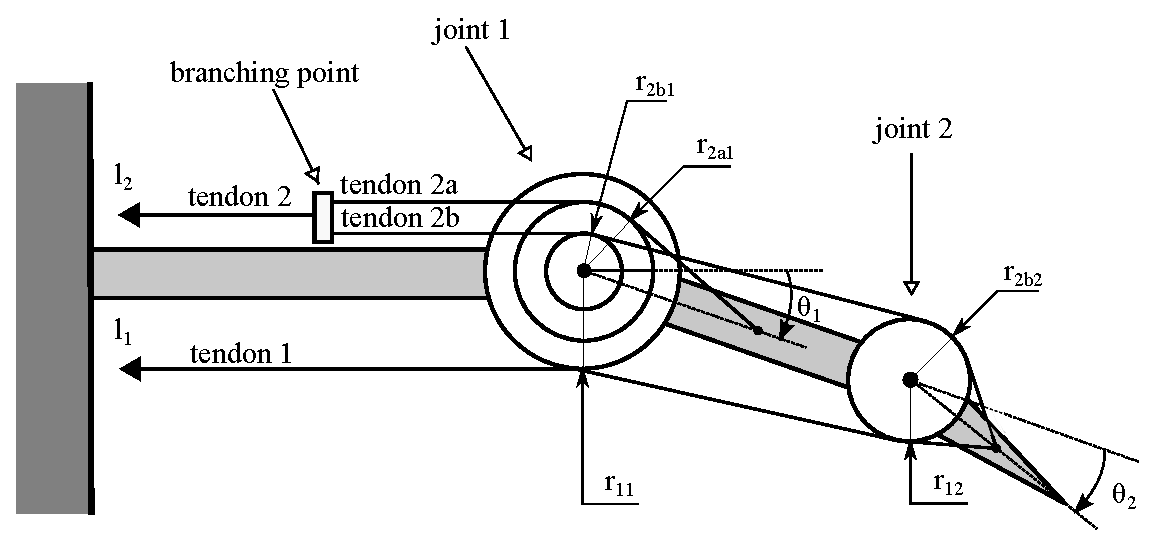
\includegraphics[width=80mm]{fig/coupled.eps}
	\caption{Robotic finger with two-DoFs and two tendons. One of the tendons branches at the branching point.}
	\label{branching_model}
\end{figure}
In the tendon-driven manipulator, the angular velocities of the joints must be related to the tendon displacement velocities.
To describe the kinematics, we must also express a general relationship between the end-point velocity and the joint angular velocities.
% In the tendon-driven manipulator, the representation of the relation between its joint angular velocities and its tendon displacement velocities is needed in addition to the general expression of the relation between its end-point velocity and its joint angular velocities to describe its kinematics.
We first relate the vector of tendon displacement velocity $\dot{\vect{l}}$ to the vector of joint angular velocity $\dot{\vect{\theta}}$ as follows:
% Given a vector of joint angular velocity $\dot{\vect{\theta}}$ and a vector of tendon displacement velocity $\dot{\vect{l}}$, the relation between them are represented as follows:
\begin{align}
	\dot{\vect{l}}=\vect{P}\dot{\vect{\theta}},
	\label{jaco}
\end{align}
where $\vect{P}$ is the tendon Jacobian matrix, determined by the routing of each tendon.
The tensile force on each tendon and joint torque are also related through the matrix $\vect{P}$:
% The relation between tensile force of each tendon and each joint torque also can be represented using with $\vect{P}$ as follows:
\begin{align}
	\vect{\tau}=-\vect{P}^{T}\vect{f},
	\label{force_relation}
\end{align}
where $\vect{\tau}$ and $\vect{f}$ are vectors of joint torques and tensile forces, respectively.
% where $\vect{\tau}$ is a vector of joint torque and $\vect{f}$ is a vector of tensile force.
If the number of tendons in the manipulator exceeds the number of joints and $\vect{P}$ is a column full-rank matrix,
the tensile force vector is expressed in terms of the joint torque vector as follows:
% In the case of that the manipulator has tendons which number is larger than joints and $\vect{P}$ is a column full-rank matrix, using with the vector of joint torque, the tensile force vector is given as
\begin{align}
	\vect{f} = -\vect{P}^{+}\vect{\tau}+\vect{f}_{b},
	\label{tensile_force}
\end{align}
where $\vect{P}^{+}$ is the pseudo-inverse of $\vect{P}$ and $\vect{f}_{b}$ is its null-space.
$\vect{f}_{b}$ is called the bias tensile force.
% More details of 
The kinematics of general tendon-driven manipulators is detailed in Kobayashi et al.\cite{kobayashi1998}
and in several robotics texts\cite{murrayi1994,tsai1999}.
\begin{figure}[t]
	\centering
	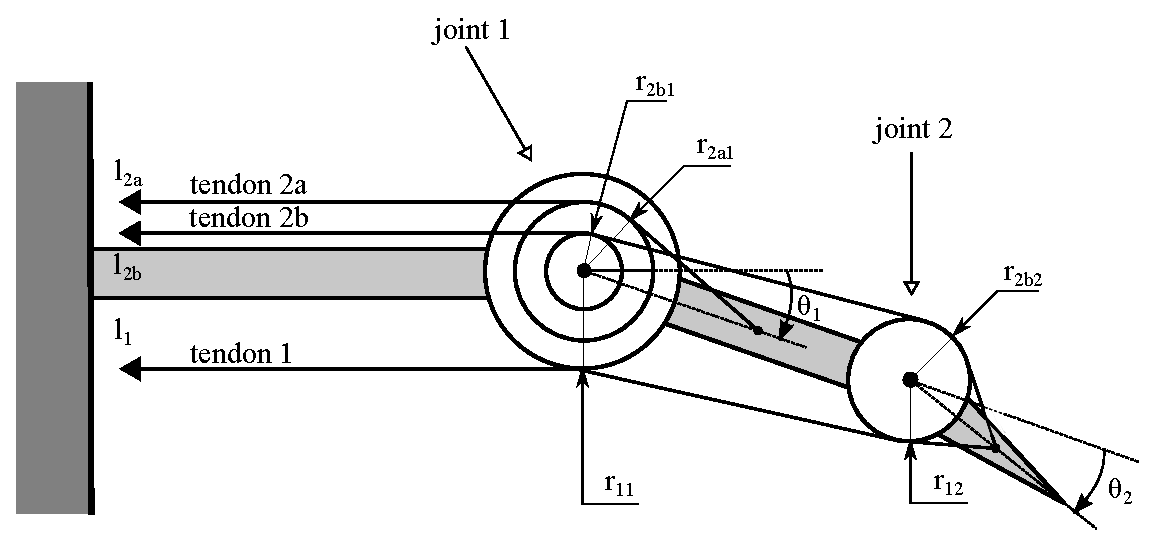
\includegraphics[width=80mm]{fig/slacked.eps}
	\caption{Model of the proposed robotic finger. The branching tendon in the proposed robotic finger can be considered as two independent tendons.}
	\label{nonbranching_model}
\end{figure}
In the proposed robotic finger, considering the branching tendon as two independent tendons, as shown in Fig. \ref{nonbranching_model}.
% Regarding the branching tendon in the proposed robotic finger as independent two tendons, the manipulator can be considered as a manipulator with three tendons as shown in Fig. \ref{nonbranching_model}.
In this case, (\ref{jaco}) can be expressed as
% represented as follows:
\begin{align}
	\begin{bmatrix}
		\dot{l}_{1}\\
		\dot{l}_{2b}\\
		\dot{l}_{2a}
	\end{bmatrix}
					=\vect{P}
					\begin{bmatrix}
					\dot{\theta}_{1}\\
					\dot{\theta}_{2}
					\end{bmatrix},
\label{jaco_relation}
\end{align}
where $l_{i}$ is
the displacement f each tendon,
% each tendon displacement, 
and the tendon Jacobian matrix is given as:
\begin{align}
	\vect{P}=
			\begin{bmatrix}
				-r_{11}&-r_{12}\\
				r_{2b1}&r_{2b2}\\
				r_{2a1}&0
			\end{bmatrix},
\label{jacobian_value}
\end{align}
where $r_{ij}$ is the moment arm between each tendon and joint (the subscript indicates the corresponding joint and tendon).
Note that the positive direction of rotation is counterclockwise in the figure,
whereas the positive tendon displacement is the pulling direction.
% and positive displacement of the tendon is in a pulling direction.
% So that any desired torque may be applied to each joint,
% the tendon control must depend on the elements of $\vect{P}$\cite{kobayashi1998}.
% We assume that $\vect{P}$ satisfies the condition of tendon controllability.
In order to apply any desired torque to each joint, the system has to be tendon controllable depending on elements of the matrix $\vect{P}$\cite{kobayashi1998}.
We assume that $\vect{P}$ is satisfied the condition to be tendon controllable.

We consider that the manipulator has a branching tendon, as shown in Fig. \ref{branching_model}
and discussed above, and investigate the kinematics.
% We consider the kinematics in the case that the manipulator has a branching tendon as Fig. \ref{branching_model} based on the expression described above.
The branching tendon has been sometimes adopted in underactuated manipulators\cite{Birglen2008}.
% The branching tendon is sometimes used to realize the underactuated manipulator\cite{Birglen2008}.
Sawada and Ozawa\cite{Sawada2012} proposed a generalized control method for a tendon-driven mechanism with branching tendons.
Shirafuji et al.\cite{Shirafuji2014b} suggested
% has been proposed 
that the tendon-driven manipulator with branching tendons can be controlled with fewer DoFs than with the original number of DoFs virtually under the assumption that the branching tendon has no elasticity.
This reduction in DoFs is caused by the geometric constraint of the branching tendon that generates coordinated joint motions.
In addition, Shirafuji et al. implied that the system can be arbitrarily released from this coupled motion by adjusting the bias tensile force.
Here, we apply Shirafuji et al.'s approach\cite{Shirafuji2014b} to our proposed robotic finger, and derive the conditions under which coupled motion is retained.

Shirafuji et al.\cite{Shirafuji2014b} use a virtual tendon Jacobian matrix $\vect{P}_v$ to represent the relationships between tendons including branched tendons and coupled joints.
First, we derive this matrix for the proposed robotic finger.
Equation (\ref{jaco_relation}) can be divided as follows:
\begin{align}
	\dot{l}_{1}&=\vect{P}_{1}
							\begin{bmatrix}
								\dot{\theta}_{1}\\
								\dot{\theta}_{2}
							\end{bmatrix},		\label{subjacobian2}\\
	\begin{bmatrix}
		\dot{l}_{2a}\\
		\dot{l}_{2b}
	\end{bmatrix}&=\vect{P}_{2}
							\begin{bmatrix}
						\dot{\theta}_{1}\\
						\dot{\theta}_{2}
							\end{bmatrix},		\label{subjacobian1}
\end{align}
where $\vect{P}_{1}$ and $\vect{P}_{2}$ are the corresponding submatrices, given as:
\begin{align}
	\vect{P}_{1}=
			\begin{bmatrix}
				-r_{11}&-r_{12}
			\end{bmatrix}
				\ 
	\vect{P}_{2}=
			\begin{bmatrix}
				r_{2b1}&r_{2b2}\\
				r_{2a1}&0
			\end{bmatrix}.			\label{subjacobian_value}
\end{align}
If neither tendon is slackened, the tendon displacement velocities of both tendons branched from tendon 1 has to be the same
because they are connected at the same point.
Therefore, $\dot{l}_{2a}=\dot{l}_{2b}=\dot{l}_{2}$ and (\ref{subjacobian1}) can be rewritten as:
\begin{align}
	\dot{l}_{2}
	\begin{bmatrix}
		1\\
		1
	\end{bmatrix}
							=\vect{P}_{2}
							\begin{bmatrix}
						\dot{\theta}_{1}\\
						\dot{\theta}_{2}
							\end{bmatrix}.
\end{align}
The joint angler velocity is derived using the inverse of $\vect{P}_{1}$ as follows:
\begin{align}
		\begin{bmatrix}
	\dot{\theta}_{1}\\
	\dot{\theta}_{2}
		\end{bmatrix}
	=\dot{l}_{2}\vect{P}_{2}^{-1}
	\begin{bmatrix}
		1\\
		1
	\end{bmatrix}
									=\frac{\dot{l}_{2}}{r_{2a1}}
									\begin{bmatrix}
									1\\
									\frac{r_{2a1}-r_{2b1}}{r_{2b2}}
									\end{bmatrix}.
\label{theta}
\end{align}
During completely taut coupled motion, the angular velocities of each joint are related as follows:
% it can be seen that the relation between each joint angular velocity is described as:
\begin{align}
	\dot{\theta}_{1}:\dot{\theta}_{2}=1:\frac{r_{2a1}-r_{2b1}}{r_{2b2}}.
\end{align}
Next, we now detail the condition under which the tendons remain taut,
and define a virtual angle $\theta_v$ that represents the angle of the coupled joints:
% The condition not to cause slackness to tendons will hereinafter be described in detail.
% We define a virtual angle $\theta_v$ to represent the angle of coupled joints as 
$\dot{\theta}_v=\dot{l}_2$.
Substituting (\ref{theta}) into (\ref{jaco_relation}), we obtain
\begin{align}
	\begin{bmatrix}
		\dot{l}_{1}\\
		\dot{l}_{2b}\\
		\dot{l}_{2a}
	\end{bmatrix}
	=
	\begin{bmatrix}
	\vect{P}_{1}\\
	\vect{P}_{2}
	\end{bmatrix}
	\dot{l}_{2}\vect{P}_{2}^{-1}
								\begin{bmatrix}
									1\\
									1
								\end{bmatrix}
								=
								\begin{bmatrix}\vect{P}_{1}\vect{P}_{2}^{-1}
																				\begin{bmatrix}
																			1\\
																			1
																				\end{bmatrix}
																			\\
								1\\
								1
								\end{bmatrix}
										\dot{\theta}_v.			\label{new_jaco_relation}
\end{align}
Since $\dot{l}_{2a}=\dot{l}_{2b}=\dot{l}_{2}$ in the absence of slack, (\ref{new_jaco_relation}) can be rewritten as follows:
\begin{align}
	\begin{bmatrix}
		\dot{l}_{1}\\
		\dot{l}_{2}
	\end{bmatrix}
	=
	\begin{bmatrix}\vect{P}_{1}\vect{P}_{2}^{-1}
													\begin{bmatrix}
												1\\
												1
													\end{bmatrix}
												\\
	1
	\end{bmatrix}
			\dot{\theta}_v.	\label{eq:l_theta_v}
\end{align}
Equation (\ref{eq:l_theta_v}) relates
% This align can be regarded as the relation between 
the joint angular velocities to the tendon displacement velocity of the tendon-driven manipulator with one-DoF and two tendons.
In this case, the tendon Jacobian matrix of the system is
% described as:
\begin{align}
	\vect{P}_{v}=
	\begin{bmatrix}
	\vect{P}_{1}\vect{P}_{2}^{-1}
								\begin{bmatrix}
									1\\
									1
								\end{bmatrix}
									\\
	1
	\end{bmatrix},
\end{align}
and we call $\vect{P}_{v}$ as virtual tendon Jacobian matrix.
Second, we apply this matrix to (\ref{force_relation}).
Multiplying both sides of (\ref{force_relation}) by $(\vect{P}_{2}^{-1}[1\ 1]^{T})^{T}$, we obtain:
\begin{align}
	\begin{bmatrix}
		1&1
	\end{bmatrix}
	\vect{P}_{2}^{-T}\vect{\tau}=-
	\begin{bmatrix}
		1&1
	\end{bmatrix}
	\vect{P}_{2}^{-T}\vect{P}^{T}\vect{f}=-\vect{P}_{v}
	\begin{bmatrix}
		f_{1}\\
		f_{2a}+f_{2b}
	\end{bmatrix},
\end{align}
where $f_{i}$ denotes the tensile forces and $f_{2a}+f_{2b}$ is equivalent to the tensile force of the branching tendon $f_{2}$.
Furthermore, defining the virtual torque vector by
\begin{align}
	\tau_{v}=
	\begin{bmatrix}
		1&1
	\end{bmatrix}
	\vect{P}_{2}^{-T}\vect{\tau},
\end{align}
we can control the proposed robotic finger regarding as a tendon-driven manipulator with one-DoF and two tendons virtually under the assuming that there is no slack of the tendons.

On the other hand, the coupled motion is lost when one of the divided tendons becomes slack.
% We assumed that there is no slack of tendon in the above discussion, but the coupled motion is lost when one of the divided tendons is slack.
Slackening is induced by the forces applied to the robotic finger, 
including the external forces generated by contact with the einvironment and inertial forces during finger motion.
% This slack is caused by forces applied to the robotic finger, include external force generated by the contact with the environment and inertial force during its motion.
The proposed robotic finger has a branching tendon, and slackness permits two states of tendons, as shown Fig. \ref{slacked_tendons}.
These states can be used for controlling the robotic finger without coupled joint motions (for instance, when the finger manipulates a grasped object using its end link).
Therefore, we finally derive a condition that one of the tendons divided from the branching tendon slackens
when an external force applied to the fingertip supplies torque to the joints.
This situation is shown in Fig. \ref{external_force}
% Finally, therefore, we derive the condition that one of the tendons divided from the branching tendon become slack when torques are applied to the joints as a result of the external force applied to the fingertip as shown in Fig. \ref{external_force}.
Considering a planar motion, and given the external force applied to the robotic fingertip by the vector $\vect{F}$,
the joint torques are related to the external force as
% the relation between the external force and joint torques can be represented as:
\begin{align}
	\vect{\tau}=\vect{J}^{T}\vect{F},
\label{standard_jacobian}
\end{align}
where $\vect{J}$ is a Jacobian matrix relating the velocity of the contact point in each direction to each joint angular velocity.
Assuming frictionless point contact, the external force vector can be described as $\vect{F}=[0\ F]^{T}$, and (\ref{standard_jacobian}) can be written as:
\begin{align}
	\vect{\tau}=
		\begin{bmatrix}
	L_{1}\cos\theta_{1}+L_{2}\cos(\theta_{1}+\theta_{2})\\
	L_{2}\cos(\theta_{1}+\theta_{2})
		\end{bmatrix}F,
\label{tau}
\end{align}
where $L_{1}$ is the length of the link between the joints and $L_{2}$ is the distance between the contact point and joint 2.
Because tendons exert no pushing motion, they slacken when their tensile force becomes negative.
% The slack of each tendon is occurred when its tensile force becomes negative because a tendon can not exert a pushing force.
Therefore, substituting (\ref{tau}) into (\ref{tensile_force}), we obtain
\begin{align}
	\begin{bmatrix}
	f_{1}\\
	f_{2b}\\
	f_{2a}
		\end{bmatrix}
	=-\vect{P}^{+}
		\begin{bmatrix}
	L_{1}\cos\theta_{1}+L_{2}\cos(\theta_{1}+\theta_{2})\\
	L_{2}\cos(\theta_{1}+\theta_{2})
		\end{bmatrix}
	F+\vect{f}_{b},	\label{eq:f-tau-pinv}
\end{align}
where the branching tendon is considered as two independent tendons (see Fig. \ref{external_force}).
% where we regard the branching tendon as independent tendons as shown Fig. \ref{external_force}.
When either $f_{2b}$ or $f_{2a}$ becomes negative under the external force $F$ and the bias force vector $\vect{f_b}$,
the corresponding tendon becomes slack, as shown in Fig. \ref{slacked_tendons},
and the coupled motion is annulled.
% When one of $f_{2b}$ and $f_{2a}$ become negative for given the external force $F$ and the bias force vector $\vect{f_{b}}$, the state of tendons change to the state such as Fig. \ref{slacked_tendons}, and this is the condition to nullify the coupled motion.
Using the relationships derived in this section, we develop the robotic finger in the next section.
We also validate the state transition of the tendons caused by the slack of tendon in the following section.
% We use these derived relations in this section to develop the robotic finger and validate the state transition of the tendons caused by the slack of tendon in the following section.

\begin{figure}[t]
	\centering
	\subfigure[]{
	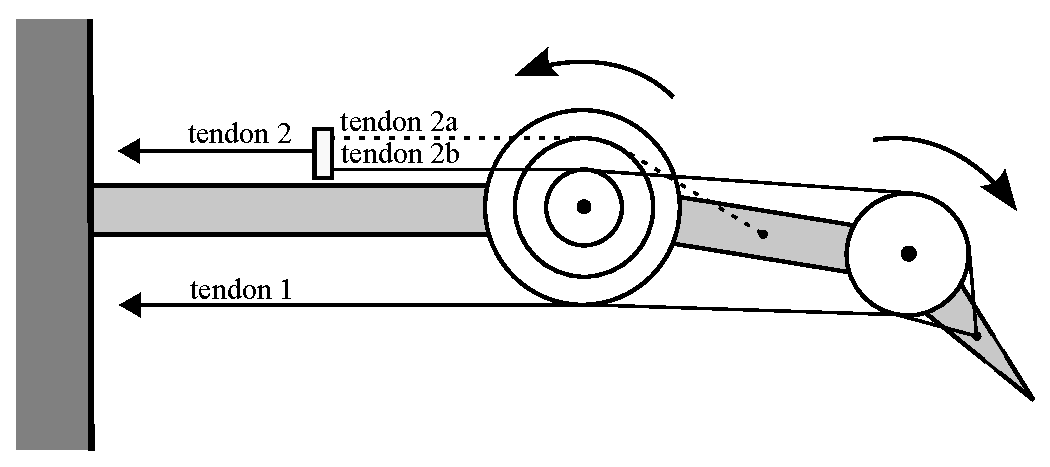
\includegraphics[width=50mm]{fig/slack1.eps}}
	% \hspace{20mm}
	\subfigure[]{
	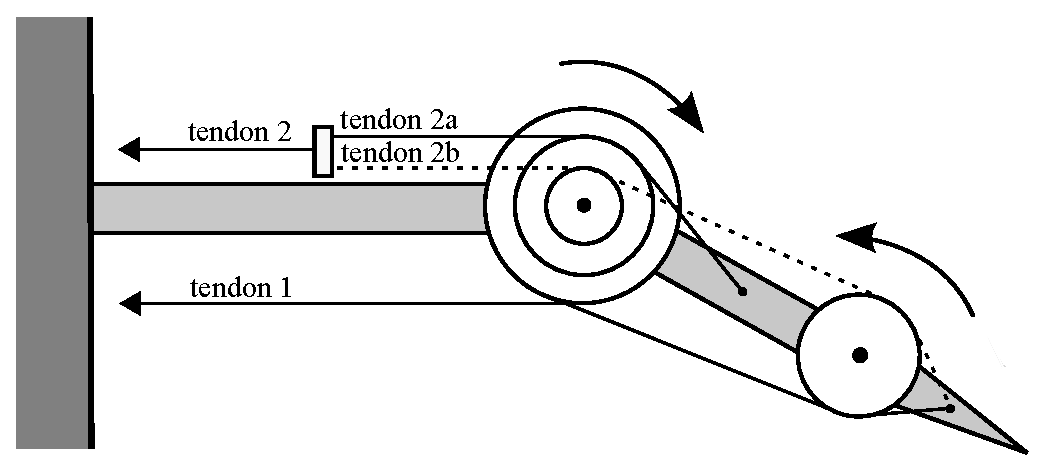
\includegraphics[width=50mm]{fig/slack2.eps}}
	\caption{States of the tendons when one tendon is slack. The slackened tendon is indicated by the dotted line. (a) The state when tendon 2a is slack. (b)  The state when tendon 2b is slack.}
	\label{slacked_tendons}
\end{figure}

\begin{figure}[t]
	\centering
	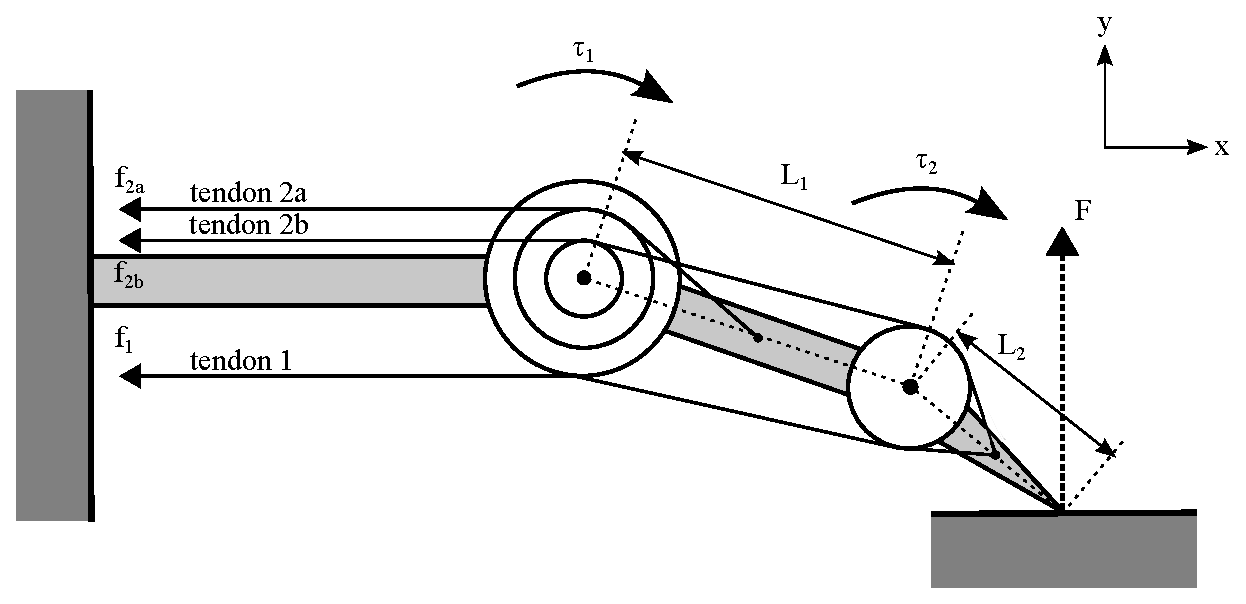
\includegraphics[width=80mm]{fig/force.eps}
	\caption{Model of force equilibrium resulting from a contact with the environment.}
	\label{external_force}
\end{figure}

% \section{robotic finger with non-elastic bifurcate tendon} % (fold)
% \label{sec:development}	
% Fig. \ref{fig:coupled} shows the developed 2DoF robotic finger driven by
% two tendons.
% % 本論文で,開発する2関節2腱のロボットフィンガのイメージを,図
% % \ref{fig:coupled}に示す.
% The finger has a non-elastic bifurcate tendon on the extensor aspect and
% the antagonist tendon is located on the flexor aspect.
% % フィンガは,伸展側に分岐腱をもち,屈曲側に拮抗に腱が存在する.
% The two branches of the bifurcate tendon connected to two linckages over
% two joints.
% % 分岐腱は,分岐した後に2つの関節を通っており,分岐前には関節を通らない.
% By reeling this tendon, these two joint are driven and they completely
% engage while the branches are tight.
% これらの腱をアクチュエータで巻き取って駆動することで,腱が通っている関節
% にトルクが発生し,フィンガを動作させることができる.
% 特に,このように分岐腱が存在するフィンガにおいて,どの腱にも緩みが生じな
% いような状態で腱を駆動すると,分岐腱が関与する関節に連動が生じる.

% この分岐腱をもつ2関節2腱のロボットフィンガを開発し,制御することを考える.

%  % \begin{figure}[tb]
%  %  \centering
%  %  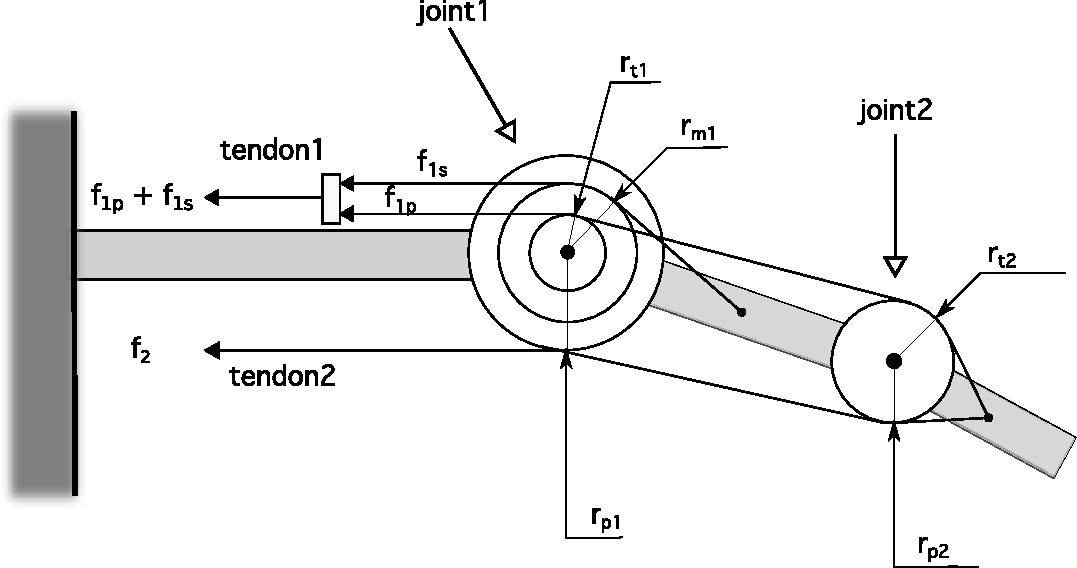
\includegraphics[width=.80\textwidth]{./figure/coupled.pdf}
%  %  \caption{分岐腱をもつ2関節2腱のロボットフィンガ}
%  %  \label{fig:coupled}
%  % \end{figure}

% 本章では,まず,一般的な腱駆動機構の運動学的表現と,分岐腱をもつ腱駆動機
% 構の運動学的表現について簡単に述べる.
% その後,実際に開発したロボットフィンガの詳細について述べる.


% \subsection{腱駆動機構における非伸縮分岐腱構造} 
%  \label{sub:branching_tendon}
% 関節を直接駆動するロボットの運動学は,関節角速度と手先の変位速度を関係づ
% けるヤコビアン行列を用いて表される.
% 腱駆動ロボットでは,これに加えて,腱の変位速度と関節角速度を関係づける腱
% ヤコビアン行列を用いて,運動が表現される.
% 分岐腱をもつロボットの場合,十分に緩みの生じない状態であるという仮定のも
% と,その幾何学的拘束により,この表現を簡略化することができる.
% 本節では,開発する2関節2腱のロボットフィンガを念頭に,腱駆動ロボットの運
% 動学的表現について述べた後,分岐腱をもつ場合にその表現がどのように変化す
% るか示す.

% \subsubsection{腱ヤコビアン} % (fold)
% \label{subsub:tendon_jacobian}
% 腱駆動ロボットフィンガの運動学的な表現を示す.
% Kobayashi et al.\cite{kobayashion1998}によると,腱駆動のロボットにおいて,
% 腱の移動速度$\bm{\dot{l}}$は,関節角速度$\bm{\dot{\theta}}$により,
		
% 		\begin{align}
% 		 \bm{\dot{l}} = \bm{J} \bm{\dot{\theta}},	\label{eq:l-theta}
% 		\end{align}
		
% 		と表される.
% 		ここで,$\bm{J}$は腱ヤコビアンであり,腱の各関節でのモーメントアームにより決定される行列である.

% 		さらにこの式と仮想仕事の原理により,各関節のトルク$\bm{\tau}$と腱の張力$\bm{f}$の間には,
		
% 		\begin{align}
% 		 \bm{\tau} = - \bm{J}^T \bm{f},	\label{eq:tau-f}
% 		\end{align}

% 		という関係が成立する.
% 		これより,腱ヤコビアン$\bm{J}$が正則であるとき,腱張力$\bm{f}$は,関節トルク$\bm{\tau}$用いて,

% 		\begin{align}
% 		 \bm{f} = - \bm{J}^{-T} \bm{\tau},	\label{eq:f-tau}
% 		\end{align}

% 		となる.
% 		しかし,実際のロボットフィンガでは,多くの場合において,腱ヤコビアンは正則ではない.
% 		このとき,$\bm{f}$は,次のように表される.

% 		\begin{align}
% 		 \bm{f} = - \bm{A}\bm{\tau} + \bm{f}_b.	\label{eq:f-tau-pinv}
% 		\end{align}

% 		ここで,$\bm{A}$は,$\bm{A} = \bm{J}(\bm{J}^T\bm{J})^{-1}$で表される$\bm{J}^T$の擬似逆行列である.
% 		$\bm{f}_b$は,$\bm{f}_b = (\bm{E} - \bm{A}\bm{J}^T)\bm{\xi}$で表されるバイアス腱張力である.
% 		$\bm{E}$は単位行列,$\bm{\xi}$は次元の一致する任意のベクトルである.
% 		式で表されるように,関節の数よりも多くの腱でフィンガを駆動する場合,$\bm{f}_b$で表されるような任意のバイアス張力を腱に加えることができる.
% 		このバイアス張力を変化させても,関節に発生するトルクは変わらない.
% 		また,腱駆動のロボットにおいては,腱で押すことはできないため,負の腱張力を発生させることはできない.
% 		そのため,腱を緩ませずにロボットを制御するためには,与えられた目標の関節トルクに対して,腱張力が正になるようなバイアス張力をかける必要がある.
% 		% (剛性について書くなら,アクチュエータと駆動軸間の非線形受動要素について言及が必要)
% 		% しかし,バイアス張力を多きくすればするほど,フィンガに外力を加えたときの動きに対する影響が小さくなる.
% 		% 逆に,バイアス張力が小さければ,外力の影響を非常に受けやすくなる.
% 		% したがって,こういったフィンガでは,関節の外力に対する動きにくさ,いわゆる剛性のようなものを自由に制御することができる.

% 		開発するフィンガにおけるヤコビアンを求める.
% 		分岐腱をそれぞれ独立の腱として考えると,2関節ロボットフィンガは図\ref{fig:finger}のようになる.
% 		ここで,関節角度,関節トルク,腱張力の各変数は,図中の矢印の向きを正とする.
% 		角度とトルクに関しては,フィンガが屈曲する向き,腱張力に関しては,腱が引っ張られる向きを正としている.
% 		また,図中には示していないが,腱の移動速度については,腱張力と同じく腱が引っ張られる向きを正とする.

% 		関節のトルクと腱張力の間の関係は,図より,各関節における腱のモーメントアームを用いて,

% 		\begin{figure}[tb]
% 		 \centering
% 		 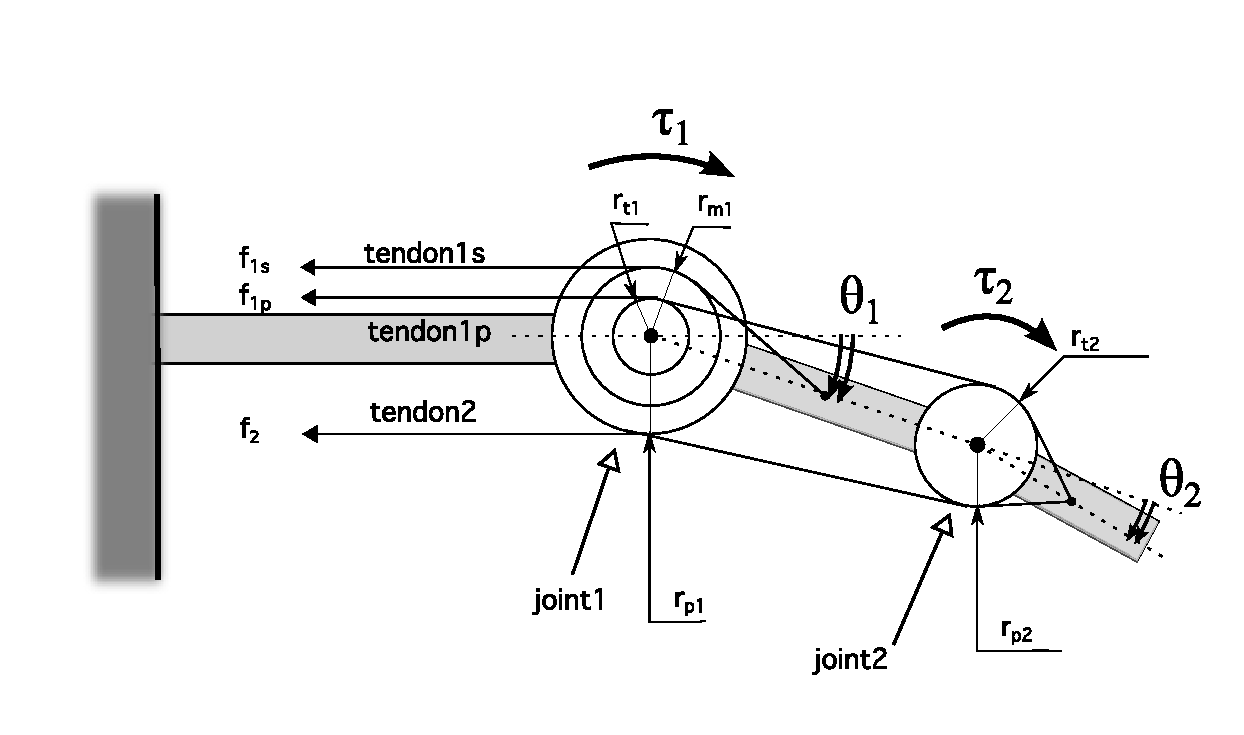
\includegraphics[width=.90\textwidth]{./figure/finger.pdf}
% 		 \caption{2関節2腱ロボットフィンガ}
% 		 \label{fig:finger}
% 		\end{figure}
		
% 		\begin{align}
% 		 \tau_1 & = r_{p1} f_2 - r_{t1} f_{1p} - r_{m1} f_{1s}, 	\label{eq:tau1-f-r}	\\
% 		 \tau_2 & = r_{p2} f_2 - r_{t2} f_{1p}, \label{eq:tau2-f-r}
% 		\end{align}
		
% 		という連立方程式として与えられる.
% 		$\tau_1,\tau_2$はそれぞれ,関節1,2におけるトルクであり,指が屈曲するときの方向を正とする.
% 				       これより,$\bm{\tau} = \begin{bmatrix}\tau_1 & \tau_2	\end{bmatrix}^T$,$\bm{f} = \begin{bmatrix}f_2 & f_{1p} & f_{1s}\end{bmatrix}^T$とおくと,式(\ref{eq:tau-f})から,$\bm{\tau}$と$\bm{f}$の関係を表す腱ヤコビアンが,次のように得られる.
							
% 				       \begin{align}
% 					\begin{bmatrix}
% 					 \tau_1	\\
% 					 \tau_2
% 					\end{bmatrix} & = 
% 					\begin{bmatrix}
% 				 	 r_{p1} & - r_{t1} & - r_{m1} \\
% 				 	 r_{p2} & - r_{t2} & 0
% 					\end{bmatrix}\begin{bmatrix}
% 						      f_2	\\
% 						      f_{1p}	\\
% 						      f_{1s}
% 						     \end{bmatrix}.	\label{eq:Jt}	\\
% 					\bm{J} & = 
% 					\begin{bmatrix}
% 					 - r_{p1} & - r_{p2} \\
% 					 r_{t1} &  r_{t2} \\
% 					 r_{m1} & 0
% 					\end{bmatrix}.	\label{eq:J}
% 				       \end{align}
							
% 				       この腱ヤコビアンを用いて,順運動学問題,逆運動学問題を考えることができる.
% 				       腱ヤコビアンから分かるように,腱駆動のロボットフィンガでは,各関節における腱のモーメントアームによって,腱張力と関節トルクの関係が変化する.
% 				       したがって,モーメントアームを変化させることにより,異なる動きのフィンガを設計することができる.

% 				       % subsection tendon_jacobian (end)

% 				       \subsection{分岐腱における仮想腱ヤコビアン} % (fold)
% 				       \label{sub:branching_tendon}
% 				       ロボットフィンガが,図\ref{fig:coupled}のような腱構造をもつ場合,式(\ref{eq:l-theta})を変形すると,

% 				       \begin{align}
% 					\begin{bmatrix}
% 					 \dot{l_{2}} \\
% 					 \dot{l_{1p}} \\
% 					 \dot{l_{1s}}
% 					\end{bmatrix} 
% 					& = 
% 					\begin{bmatrix}
% 					 \bm{J}_2 \\
% 					 \bm{J}_1
% 					\end{bmatrix} 
% 					\begin{bmatrix}
% 					 \dot{\theta_1} \\
% 					 \dot{\theta_2}
% 					\end{bmatrix}, \label{eq:l-theta_2joint}
% 				       \end{align}

% 				       が得られ,これを展開すると,

% 				       \begin{align}
% 					\begin{bmatrix}
% 					 \dot{l_{2}} \\
% 					 \begin{bmatrix}
% 					  \dot{l_{1p}} \\
% 					  \dot{l_{1s}}
% 					 \end{bmatrix}
% 					\end{bmatrix} 
% 					& = 
% 					\begin{bmatrix}
% 					 \bm{J}_2 
% 					 \begin{bmatrix}
% 					  \dot{\theta_1} \\
% 					  \dot{\theta_2}
% 					 \end{bmatrix} \\
% 					 \bm{J}_1
% 					 \begin{bmatrix}
% 					  \dot{\theta_1} \\
% 					  \dot{\theta_2}
% 					 \end{bmatrix}
% 					\end{bmatrix}, \label{eq:l-theta_branching}
% 				       \end{align}

% 				       という関係式が得られる.
% 				       $\dot{l_2},\dot{l_{1p}},\dot{l_{1s}}$はそれぞれ,腱2と,腱1が分岐したあとの,腱1p,腱1sの移動速度であり,$\dot{\theta_1},\dot{\theta_2}$は,関節1,2の角速度である.
% 				       ここで,$\bm{J}_2$は1×2行列,$\bm{J}_1$は2×2行列で,それぞれが腱2,1に対応する腱ヤコビアン$\bm{J}$の部分行列である.
% 				       \begin{align}
% 					\bm{J}_2 = 
% 					\begin{bmatrix}
% 					 - r_{p1} & - r_{p2}
% 					\end{bmatrix}, 
% 					\bm{J}_1 = 
% 					\begin{bmatrix}
% 					 r_{t1} &  r_{t2} \\
% 					 r_{m1} & 0
% 					\end{bmatrix}.	\label{eq:component_J}
% 				       \end{align}

% 				       ここで,腱の移動速度$\bm{\dot{l}} = \begin{bmatrix}
% 									    \dot{l_{2}} & \dot{l_{1p}} & \dot{l_{1s}}			
% 									   \end{bmatrix}^T $について,分岐した腱のどちらにも緩みがないときには,$\dot{l_{1p}} = \dot{l_{1s}}$が成り立つ.
% 									   これを用いて,式(\ref{eq:l-theta_branching})の腱1に関する部分を展開する.
% 									   まず,腱1に関する部分は,$\dot{l_{1p}} = \dot{l_{1s}}$のとき,

% 									   \begin{align}
% 									    \begin{bmatrix}
% 									     \dot{l_{1p}} \\
% 									     \dot{l_{1p}}
% 									    \end{bmatrix} 
% 									    & = 
% 									    \bm{J}_1
% 									    \begin{bmatrix}
% 									     \dot{\theta_1} \\
% 									     \dot{\theta_2}
% 									    \end{bmatrix},
% 									   \end{align}

% 									   と表される.
% 									   $\bm{J}_1$は,式(\ref{eq:component_J})より正則なので,逆行列が存在する.
% 									   よって,逆行列により,関節角速度$\dot{\bm{\theta}}$が計算でき,

% 									   \begin{align}
% 									    \begin{bmatrix}
% 									     \dot{\theta_1} \\
% 									     \dot{\theta_2}
% 									    \end{bmatrix} 
% 									    & = \dot{l_{1p}} \bm{J}_1^{-1} 
% 									    \begin{bmatrix}
% 									     1 \\
% 									     1
% 									    \end{bmatrix}, \label{eq:theta_coupled}
% 									   \end{align}

% 									   となる.
% 									   ここで,式(\ref{eq:component_J})より,$\bm{J}_1$をモーメントアームを用いて表すと,$\dot{\bm{\theta}}$は,

% 									   \begin{align}
% 									    \begin{bmatrix}
% 									     \dot{\theta_1} \\
% 									     \dot{\theta_2}
% 									    \end{bmatrix} 
% 									    & = - \frac{\dot{l_{1p}}}{r_{m1}r_{t2}}
% 									    \begin{bmatrix}
% 									     0 & -r_{t2} \\
% 									     -r_{m1} & r_{t1}
% 									    \end{bmatrix}
% 									    \begin{bmatrix}
% 									     1 \\
% 									     1
% 									    \end{bmatrix}, \\
% 									    \begin{bmatrix}
% 									     \dot{\theta_1} \\
% 									     \dot{\theta_2}
% 									    \end{bmatrix} 
% 									    & = \frac{\dot{l_{1p}}}{r_{m1}}
% 									    \begin{bmatrix}
% 									     1 \\
% 									     \frac{r_{m1}-r_{t1}}{r_{t2}} \label{eq:branching_theta}
% 									    \end{bmatrix},			
% 									   \end{align}

% 									   と計算できる.

% 									   以上より,2関節2腱のグリッパで分岐腱が連動しているとき,関節2と関節3の間の角速度の間に,
											
% 									   \begin{align}
% 									    \dot{\theta_1} : \dot{\theta_2} = 1 : \frac{r_{m1}-r_{t1}}{r_{t2}}, \label{eq:rate_theta}
% 									   \end{align}
											
% 									   という比例関係があることがわかる.
% 									   また,式(\ref{eq:branching_theta})の右辺に含まれる時間に依存する項は$\dot{l_{1p}}$のみであるので,関節の角度についても,初期姿勢の角度の値を上手く定義することで,同様の比例関係が成り立つ.

% 									   このように,分岐腱をもつロボットフィンガにおいては,分岐腱に緩みがなければ,分岐腱が関与する関節は,連動することが分かる.
% 									   したがって,関節を連動させた状態で制御したい場合には,分岐腱が緩まないように注意する必要がある.
% 									   この分岐腱が緩む条件については,後述する.
% 									   % 特に,腱に張力がかかっているフィンガが物体に接触しておらず,外力が働いていない場合,腱は緩まないため,関節の連動が必ず生じる.

% 									   この連動が生じているとき,$\dot{\bm{\theta}}$は,上述のように,式(\ref{eq:theta_coupled})で表される.
% 									   これを,式(\ref{eq:l-theta_2joint})の$\dot{\bm{\theta}}$に代入し式を変形すると,

% 									   \begin{align}
% 									    \begin{bmatrix}
% 									     \dot{l_{2}} \\
% 									     \dot{l_{1p}} \\
% 									     \dot{l_{1s}}
% 									    \end{bmatrix} 
% 									    & = 
% 									    \begin{bmatrix}
% 									     \bm{J}_2 \\
% 									     \bm{J}_1
% 									    \end{bmatrix} 
% 									    \dot{l_{1p}} \bm{J}_1^{-1} 
% 									    \begin{bmatrix}
% 									     1 \\
% 									     1
% 									    \end{bmatrix}, \label{eq:leading_Jc}	\\	
% 									    % \begin{bmatrix}
% 									    % 	\dot{l_{2}} \\
% 									    % 	\dot{l_{1p}} \\
% 									    % 	\dot{l_{1s}}
% 									      % \end{bmatrix} 
% 									    %  & = \dot{l_{1p}}
% 									    %  \begin{bmatrix}
% 									    %  	\bm{J}_2 \bm{J}_1^{-1} 
% 									    %  \begin{bmatrix}
% 									    % 	1 \\
% 									    % 	1
% 									       %  \end{bmatrix}	\\
% 									    %  	\bm{J}_1 \bm{J}_1^{-1} 
% 									    %  \begin{bmatrix}
% 									    % 	1 \\
% 									    % 	1
% 									       %  \end{bmatrix}
% 									       %  \end{bmatrix}, \\
% 									    \begin{bmatrix}
% 									     \dot{l_{2}} \\
% 									     \begin{bmatrix}
% 									      \dot{l_{1p}} \\
% 									      \dot{l_{1s}}
% 									     \end{bmatrix}
% 									    \end{bmatrix} 
% 									    & = \dot{l_{1p}}
% 									    \begin{bmatrix}
% 									     \bm{J}_2 \bm{J}_1^{-1} 
% 									     \begin{bmatrix}
% 									      1 \\
% 									      1
% 									     \end{bmatrix}	\\
% 									     \begin{bmatrix}
% 									      1 \\
% 									      1
% 									     \end{bmatrix}
% 									    \end{bmatrix},
% 									   \end{align}

% 									   となる.
% 									   右辺の行列において,腱1に相当する下側2行は線形従属となっている.
% 									   これをまとめた行列を$\bm{J}_c$とおくと,

% 									   \begin{align}
% 									    \bm{J}_c &= 
% 									    \begin{bmatrix}
% 									     \bm{J}_2 \bm{J}_1^{-1}
% 									     \begin{bmatrix}
% 									      1 \\
% 									      1
% 									     \end{bmatrix} \\
% 									     1
% 									    \end{bmatrix},
% 									   \end{align}

% 									   となる.
% 									   この行列$\bm{J}_c$を,仮想腱ヤコビアンと呼び,分岐腱をもつロボットフィンガにおいて,その運動を記述する際に用いることができる.

% 									   この仮想腱ヤコビアンを,式(\ref{eq:tau-f})においても利用することを考える.
% 																												 式(\ref{eq:tau-f})のヤコビアン$\bm{J}$を,$\bm{J}_c$に変換するためには,式(\ref{eq:leading_Jc})における操作と同様に,ヤコビアンに右から$(\bm{J}_1^{-1}\begin{bmatrix}1 & 1\end{bmatrix}^T)^T$をかければよい.
% 																																   したがって,$(\bm{J} \bm{J}_1^{-1}\begin{bmatrix}1 & 1\end{bmatrix}^T)^T = \begin{bmatrix}1 & 1\end{bmatrix} \bm{J}_1^{-T} \bm{J}^T$より,式(\ref{eq:tau-f})の両辺に左から$\begin{bmatrix}1 & 1\end{bmatrix} \bm{J}_1^{-T}$をかけると,

% 																																   \begin{align}
% 																																    \begin{bmatrix}
% 																																     1 & 1
% 																																    \end{bmatrix} \bm{J}_1^{-T} \bm{\tau} &= - \begin{bmatrix}
% 																																						1 & 1
% 																																					       \end{bmatrix} \bm{J}_1^{-T} \bm{J} \bm{f},	\\
% 																																    \begin{bmatrix}
% 																																     1 & 1
% 																																    \end{bmatrix} \bm{J}_1^{-T} \bm{\tau} &= - (\bm{J} \bm{J}_1^{-1}
% 																																    \begin{bmatrix}
% 																																     1 \\
% 																																     1
% 																																    \end{bmatrix})^T \bm{f},
% 																																   \end{align}

% 																																   となる.
% 																																   さらに右辺を展開していくと,

% 																																   \begin{align}
% 																																    \begin{bmatrix}
% 																																     1 & 1
% 																																    \end{bmatrix} \bm{J}_1^{-T} \bm{\tau} &= - 
% 																																    \begin{bmatrix}
% 																																     (\bm{J}_2 \bm{J}_1^{-1} 
% 																																     \begin{bmatrix}
% 																																      1 \\
% 																																      1
% 																																     \end{bmatrix})^T & 
% 																																     \begin{bmatrix}
% 																																      1 & 1
% 																																     \end{bmatrix}
% 																																    \end{bmatrix} 
% 																																    \begin{bmatrix}
% 																																     f_2 \\
% 																																     f_{1p} \\
% 																																     f_{1s}
% 																																    \end{bmatrix},	\\
% 																																    \begin{bmatrix}
% 																																     1 & 1
% 																																    \end{bmatrix} \bm{J}_1^{-T} \bm{\tau} &= - 
% 																																    \begin{bmatrix}
% 																																     (\bm{J}_2 \bm{J}_1^{-1} 
% 																																     \begin{bmatrix}
% 																																      1 \\
% 																																      1
% 																																     \end{bmatrix})^T & 1
% 																																    \end{bmatrix}
% 																																    \begin{bmatrix}
% 																																     f_2 \\
% 																																     f_{1p} + f_{1s}
% 																																    \end{bmatrix},	\\
% 																																    \begin{bmatrix}
% 																																     1 & 1
% 																																    \end{bmatrix} \bm{J}_1^{-T} \bm{\tau} &= - \bm{J}_c^T
% 																																    \begin{bmatrix}
% 																																     f_2 \\
% 																																     f_{1p} + f_{1s}
% 																																    \end{bmatrix},			
% 																																   \end{align}

% 																																   と変形できる.
% 																																   ここで,左辺のベクトルは仮想腱ヤコビアンに対応するトルクを表すので,これを,

% 																																   \begin{align}
% 																																    \bm{\tau_c} &= \begin{bmatrix}
% 																																		    1 & 1
% 																																		   \end{bmatrix} \bm{J}_1^{-T} \bm{\tau}, 
% 																																   \end{align}

% 																																   とおき,$\bm{\tau_c}$を仮想トルクベクトルと呼ぶ.
% 																																   これにより,分岐腱をもつフィンガにおいても,式(\ref{eq:tau-f})と同様に,

% 																																   \begin{align}
% 																																    \bm{\tau_c} &= -\bm{J}_c^T \bm{f}, 
% 																																   \end{align}

% 																																   という形が成り立つ.

% 																																   このように,分岐腱による関節間の連動が生じているとき,トルクベクトル$\bm{\tau}$と腱張力ベクトル$\bm{f}$は,次元が1減少する.
% 																																   従って,関節角度や関越トルクといったフィンガの動きを表す値を制御における目標値とする場合,その次元も減少し,関節数よりも少ない次元の変数で,制御を行うことができる.

% 																																   % subsection branching_tendon (end)

% 																																   \subsection{分岐腱の緩み条件} % (fold)
% 																																   \label{sub:tendon_slack}
% 																																   \ref{sub:branching_tendon}で述べたように,分岐腱をもつロボットフィンガは,外力が働いていないとき,その関節が連動して動く.
% 																																   この連動は,フィンガの分岐腱の片方が緩んだときには,生じない.

% 																																   分岐腱をもつロボットフィンガは,物体との拘束によって生じる外力や自身の慣性力などの力を受けているとき,分岐腱のどちらか片方に緩みが生じることがある.
% 																																   2関節2腱のフィンガにおいては,分岐腱が1本存在するので,指先が外力を受けている場合の緩みの状態としては,図\ref{fig:tendon_slack}のような2つの状態が考えられる.
% 																																   このように物体に対する指先の姿勢を変化させることで,ピンチングにおける安定把持や,指先における細かな物体操作が,実現できると考えられる.
% 																																   また,指先でなく,関節1と関節2の間のリンクに外力がかかった場合にも,当然ながら,腱の緩みは発生することが考えられる.
% 																																   このとき,フィンガに把持方向に力を加えると,図\ref{fig:slack_tendon1s}と同じ状態になると予測される.

% 																																   ここでは,図\ref{fig:tendon_slack}のように,指先が物体で拘束されたときの分岐腱の緩み条件について,静力学的に計算する.

% 																																   \begin{figure}[tb]
% 																																    \centering
% 																																    \subfigure[]{\includegraphics*[width=.48\textwidth]{./figure/coupled.pdf}}\\
% 																																    \subfigure[\label{fig:slack_tendon1s}]{\includegraphics*[width=.48\textwidth]{./figure/uncoupled1.pdf}}
% 																																    \subfigure[\label{fig:slack_tendon1p}]{\includegraphics*[width=.48\textwidth]{./figure/uncoupled2-2.pdf}}
% 																																    \caption{分岐腱の緩み状態}
% 																																    \label{fig:tendon_slack}
% 																																   \end{figure}
																																		
% 																																   分岐腱の緩みは,フィンガの指先が物体から受ける反力と腱の張力の関係により,腱の張力を正に保てなくなることで起きる.
% 																																   まず,フィンガにより指先に発生する力$\bm{s}$は,

% 																																   \begin{align}
% 																																    \bm{\tau} &= \bm{J}_r^T \bm{s}, \label{eq:tau-s}
% 																																   \end{align}

% 																																   という関係を満たす.
% 																																   $\bm{J}_r$は,マニピュレータの手先速度$\dot{\bm{r}}$と,関節の角速度$\dot{\bm{\theta}}$を関連づけるヤコビアン行列で,

% 																																   \begin{align}
% 																																    \dot{\bm{r}} &= \bm{J}_r \dot{\bm{\theta}},
% 																																   \end{align}

% 																																   を満たす行列である.

																																		
% 																																   \begin{figure}[tb]
% 																																    \centering
% 																																    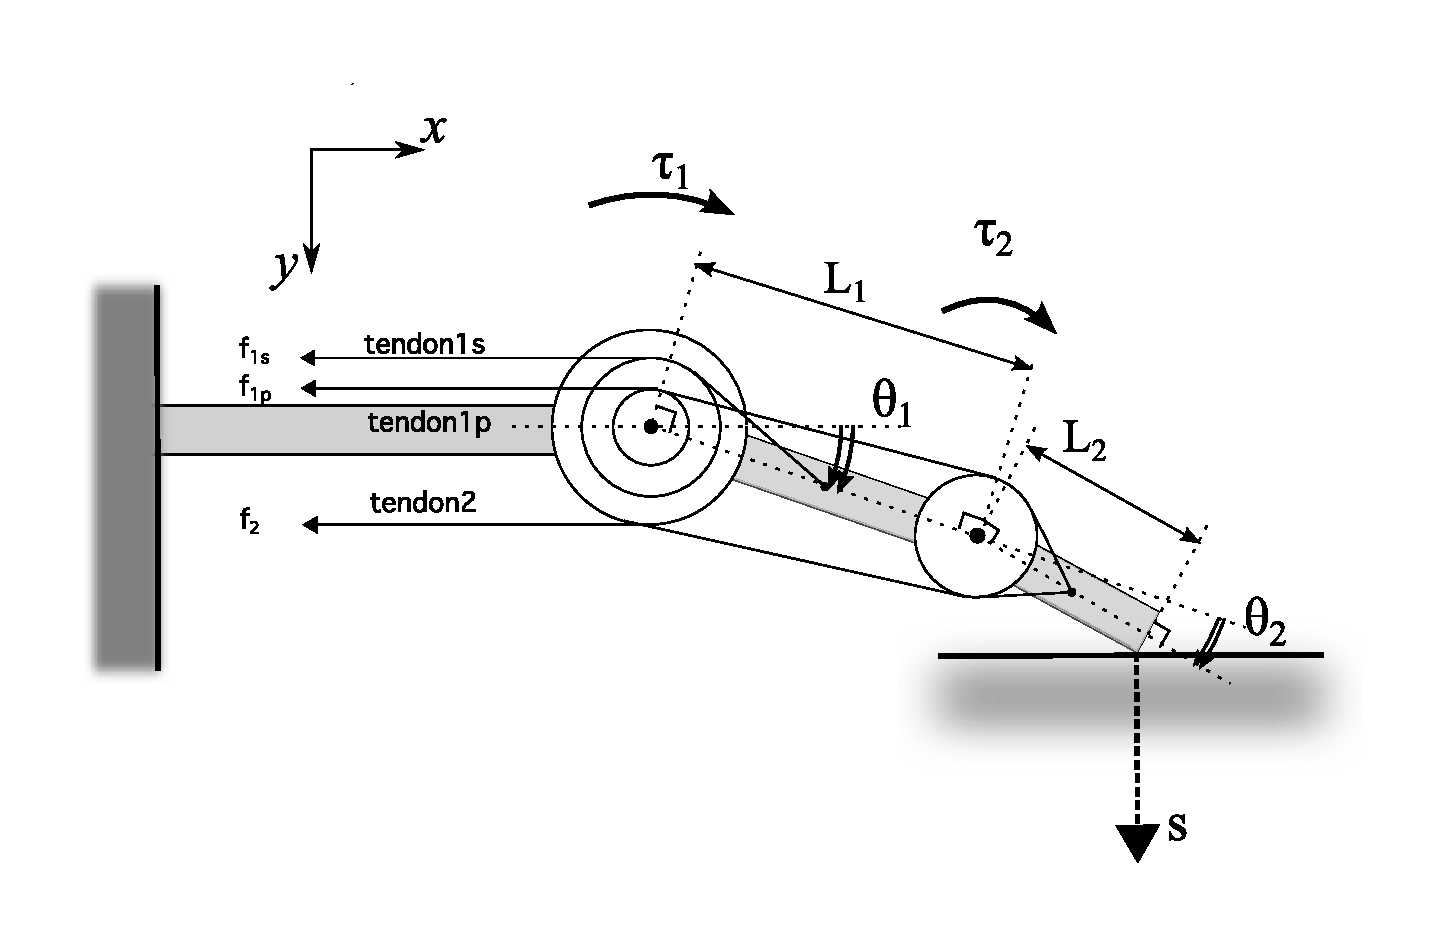
\includegraphics[width=.90\textwidth]{./figure/finger-slack.pdf}
% 																																    \caption{物体との接触}
% 																																    \label{fig:finger_slack}
% 																																   \end{figure}
																																		

% 																																   ここで,フィンガの運動を2次元に限定し,フィンガがまっすぐ伸びているときを$\theta_1,\theta_2 = 0$とし,フィンガの指先方向をx軸,矢状面上でその垂直方向をy軸とする(図\ref{fig:finger_slack}).
% 																																   このとき,静力学における$\bm{J}_r$は,

% 																																   \begin{align}
% 																																    \bm{J}_r = \begin{bmatrix}
% 																																		-(L_1\sin\theta_1 + L_2\sin(\theta_1+\theta_2)) & -L_2\sin(\theta_1+\theta_2) \\
% 																																		(L_1\cos\theta_1 + L_2\cos(\theta_1+\theta_2)) & L_2\cos(\theta_1+\theta_2)
% 																																	       \end{bmatrix},
% 																																   \end{align}

% 																																   と求まる.
% 																																   $L_1$は,関節1,2間の長さ,$L_2$は関節2と指先間の距離である.

% 																																   今,フィンガの関節が連動したまま,指先が物体に接触している状態で,指先に力を発生させることを考える.
% 																																   簡単のため,フィンガと物体の接触面には摩擦が存在しないと仮定する.
% 																																   このとき,指先にy軸方向の力しか発生していなければ,フィンガの関節は動かない.
% 																																   この,y軸方向のある力を$s$とすると,
% 																																   $\bm{s} = \begin{bmatrix}
% 																																	      0 & s
% 																																	     \end{bmatrix}^T$となる.
% 																																	     このような力を発生させる関節トルクは,式(\ref{eq:tau-s})を用いて,

% 																																	     \begin{align}
% 																																	      \bm{\tau} &= \begin{bmatrix}
% 																																			    L_1 \cos{\theta_1} + L_2 \cos(\theta_1 + \theta_2)	\\
% 																																			    L_2 \cos(\theta_1 + \theta_2)
% 																																			   \end{bmatrix} s,
% 																																	     \end{align}
																																			
% 																																	     と求めることができる.
% 																																	     腱が独立に動かせるとき,この関節トルクを発生させる腱張力は,式(\ref{eq:f-tau-pinv})より,計算で求めることができ,

% 																																	     \begin{align}
% 																																	      \bm{f} = -\bm{A} \begin{bmatrix}
% 																																				L_1 \cos\theta_1 + L_2 \cos(\theta_1 + \theta_2)	\\
% 																																				L_2 \cos(\theta_1 + \theta_2)
% 																																			       \end{bmatrix} s + \bm{f}_b	\label{eq:slack-f}
% 																																	     \end{align}

% 																																	     と求まる.
% 																																	     この式により求まった腱張力が負になる場合,そのような腱張力は発生させることができない.
% 																																	     そのため,腱張力ベクトルの成分が負になるようなバイアス張力とフィンガが出す力$s$,関節角度が与えられたとき,負となった成分に対応する腱が緩むことになる.
% 																																	     これが腱の緩む条件となる.

% 																																	     緩む条件を満たしたトルク,バイアス張力を,分岐腱により連動している状態のフィンガの制御式に与えると,腱が緩み,関節の連動が生じなくなると考えられる.
% 																																	     ここで,1自由度のフィンガは,物体と接触すると,本来はそれ以上の動きはできないため,物体から受ける力は物体の垂直方向だけである.
% 																																	     分岐腱により関節が連動している状態のフィンガは,仮想的に1自由度とみなせるので,物体と接触しているとき,x軸方向には動かず,力が発生しない.
% 																																	     そのため,フィンガの指先には,想定したようなy軸方向の力のみが発生し,腱張力は,計算通りにかかると考えられる.
																																			
% 																																	     % subsection tendon_slack (end)

% 																																	     % section branching_tendon (end)



\section{Development of Robotic Finger} % (fold)
\label{sec:producing}
	
We produced a robotic finger with a non-elastic branching tendon and assembled two developed fingers into a two-fingered gripper.
Each finger has three links and two joints with five pulleys, and is driven by flexion/extension wires.

%  \section{2関節ロボットフィンガシステム} % (fold)
%  \label{sec:producing}
% 	実際に,グリッパを開発するため,分岐腱をもつ2関節2腱のロボットフィンガを製作した.
% 	本節では,フィンガのハードウェア仕様について言及し,その仕様に基づいて,\ref{sec:branching_tendon}節で述べたヤコビアンの具体的な値を記述する.
% 	その後,制御システムとフィンガの実際の動作について述べる.

% 	  \subsection{各関節のモーメントアームと可動域} % (fold)
% 	  \label{sub:moment_arm}
Movement of the joints is determined by the applied torque, which is a function of the moment arm of each tendon.
Therefore, the moment arm is an important factor in designing the joint movement.
The finger is a simple model of a human finger, driven by branching extensor tendons and flexor tendons.
% 		\ref{sub:branching_tendon}項で述べたように,フィンガの動きや関節間の連動の比率は,各腱の各関節に対するモーメントアームによって異なる.
% 		そのため,モーメントアームの決定は,フィンガの動作を決定する重要な事項である.
% 		開発するフィンガは,指先2関節を屈曲側の腱1本と伸展側の分岐腱1本で駆動する.
% 		この構造は,ヒトの指の先端2関節と類似する部分があり,ヒトの指における腱のモーメントアームを参考にすることが考えられる.
% 		モーメントアームの設定は,Leijnse et al.\cite{Leijnse1995},Spoor\cite{Spoor1983}の示したヒトの指におけるモーメントアームを参考にして行った.
% 		実際に採用した値を,表\ref{tab:pulley}に示す.
% Table \ref{tab:pulley} shows the actual moment arms for the robotic finger, taking the real parameters into account\cite{Leijnse1995,Spoor1983}.
Based on real parameters\cite{Leijnse1995,Spoor1983}, the moment arms for the robotic finger were decided as follows:
 % The actual moment arms for the rovotic finger are decided as follows: 
 $r_{11}=7$, $r_{12}=4$, $r_{2b1}=3$, $r_{2b2}=4$, $r_{2a}=5$(units are mm).
% taking the real parameters into account\cite{Leijnse1995,Spoor1983}.
Although the moment arm $r_{2b1}$ is a nonlinear function of the PIP joint angle
% according to Leijnse et al. 
\cite{Leijnse1995}, we regard it as a constant for simplicity.
% we set it as a constant value for simplicity.
The diameter of the pulleys
was decided from real moment arms, and the link lengths also imitate those of a human finger.
% are designed depending on the real moment arms.
% 		ただし,腱1の関節1におけるモーメントアーム$r_{t1}$について,Leijnse et al.によると,このモーメントアームは,ある条件を満たすような,PIP関節の関節角度に関する非線形な関数であらわされる.
% 		Shirafuji et al.は,この非線形なモーメントアームを複数のプーリを配置することで再現しているが,本研究では,構造の簡潔化のためにこのモーメントアームは定数としている.
% 		これらのモーメントアームは各関節に腱ごとに配置されたプーリの半径によって実現されている.
% Link length is also designed to imitated a real human(Table \ref{tab:system}).
% Link length is also designed to imitated a real human.
The lengths between joint 1 and joint 2
and between joint 2 and the fingertip are 30.5 mm and 22 mm, respectively.
 % is 30.5[mm] and the length between joint 2 and fingertip is 22[mm].
% 		また,各関節間の距離は,指先の軌道や指先に発生する力に関係する.
% 		フィンガの各部分の長さを表\ref{tab:system}に示す.
		
% \begin{table}[htbp]
% 	\centering
% 	\begin{tabular}{cc}
% 		\begin{minipage}{0.5\hsize}
% 			\centering
% 			\caption{Diameters of the pulleys[mm]}
% 			\label{tab:pulley}
% 			\begin{tabular}{|c||c|c|c|} \hline
% 					& tendon 1 & tendon 2b & tendon 2a \\ \hline\hline
% 				joint 1 & $ r_{11}$ & $ r_{2b1}$ & $ r_{2a1}$ \\
% 					& 7 & 3 & 5 \\ \hline
% 				joint 2 & $ r_{12}$ & $ r_{2b2}$ & - \\
% 					& 4 & 4 & - \\ \hline
% 			\end{tabular}
% 		\end{minipage}
% 		\begin{minipage}{0.5\hsize}
% 			\centering
% 			\caption{Lengths of links[mm]}
% 			\label{tab:system}
% 			\begin{tabular}{|c||c|} \hline
% 				parts & length \\ \hline\hline
% 				fingertip - joint 2 & 22 \\
% 				joint 2 - joint 1 & 30.5 \\ \hline
% 			\end{tabular}
% 		\end{minipage}
% 	\end{tabular}
% \end{table}

% \begin{table}[htbp]
% 	\centering
% 	\caption{Diameter of the pulleys[mm]}
% 	\label{tab:pulley}
% 	\begin{tabular}{|c||c|c|c|} \hline
% 			& tendon 1 & tendon 2b & tendon 2a \\ \hline\hline
% 		joint 1 & $ r_{11}$ & $ r_{2b1}$ & $ r_{2a1}$ \\
% 			& 7 & 3 & 5 \\ \hline
% 		joint 2 & $ r_{12}$ & $ r_{2b2}$ & - \\
% 			& 4 & 4 & - \\ \hline
% 	\end{tabular}
% \end{table}

% 		\begin{table}[htbp]
% 		 \centering
% 		 \caption{フィンガの各部分の長さ[mm]}
% 		 \label{tab:system}
% 		 \begin{tabular}{|c||c|} \hline
% 		  部分 & 長さ \\ \hline\hline
% 		  指先-関節2 & 22 \\
% 		  関節2-関節1 & 30.5 \\ \hline
% 		  関節1-根元 & 45 \\
% 		  フィンガ1の根元-フィンガ2の根元 & 92 \\ \hline
% 		 \end{tabular}
% 		\end{table}

% This finger's Jacobiann defined with the diameter of pulleys as follows:
% % 		このフィンガにおけるヤコビアンは,式\ref{eq:J}で表されるので,表\ref{tab:pulley}を用いると,

% 		\begin{align}
% 			\bm{J} = \begin{bmatrix}
% 					-7 & -4 \\
% 					3 & 4	\\ 
% 					5 & 0
% 				\end{bmatrix},\label{eq:J_value}
% 		\end{align}

% % 		と求められる.

% Using these moment arms, this finger's tendon Jacobian matrix is defined and we can control the finger with the Jacobian.
% Also, the ratio between the changes in the joint angle vector shown by (\ref{theta}) is calculated as follows:
% 		% また,実際に設計に用いた値を使って,式(\ref{eq:rate_theta})に示される関節の角速度の比を計算すると,以下のようになる.
% 		\begin{align}
% 			\dot{\theta_1} : \dot{\theta_2} & = 1 : \frac{r_{2a1}-r_{2b1}}{r_{2b2}} %\nonumber\\
% 			% & = 1 : \frac{r_{m1}-r_{t1}}{r_{t2}} \\ \nonumber
% 			= 1 : \frac{1}{2}. \nonumber
% 		\end{align}

% Fig. \ref{fig:trajectory} shows the fingertip trajectory of developed finger.
% % 		また,このとき,フィンガを空中で動かした場合の指先の軌道は図\ref{fig:trajectory}のようになる.
% % 		原点は関節1の中心で,指は始め横軸正の方向に伸びている.
		
% 	\begin{figure}[tb]
% 		\centering
% 		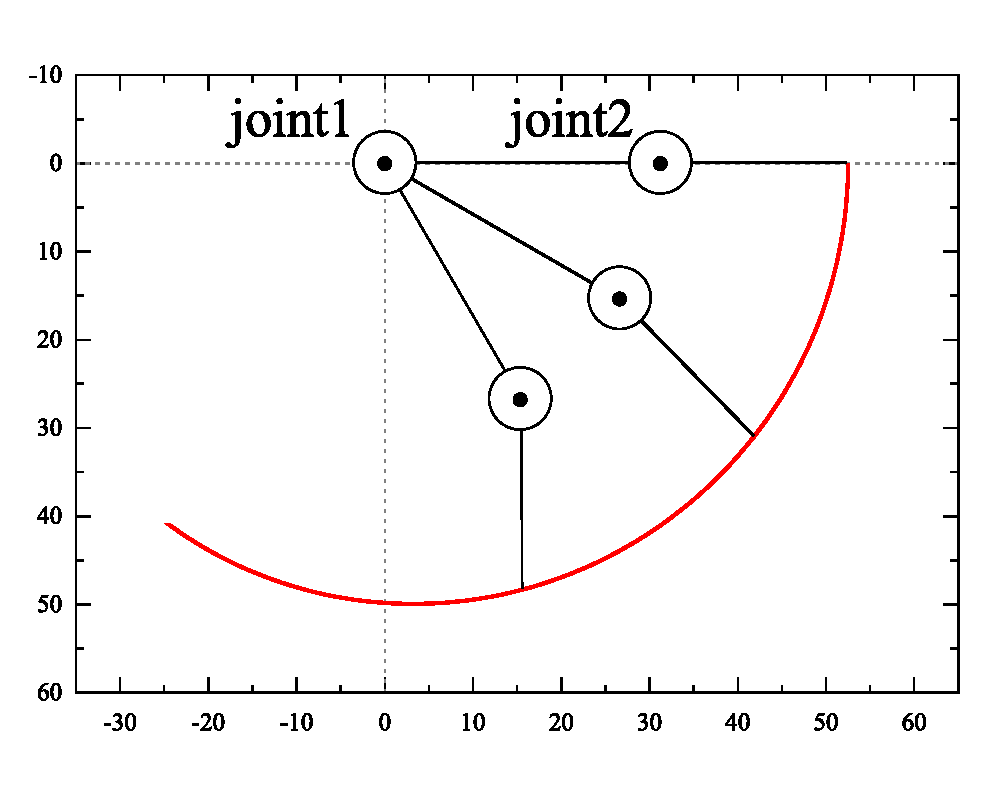
\includegraphics[width=.60\textwidth]{./figure/trajectory2.pdf}
% 		\caption{2関節フィンガの指先の軌道(横軸,縦軸とも単位は[mm])}
% 		\label{fig:trajectory}
% 	\end{figure}


% Table  shows the passive ranges of motion of each joints which is restricted mechanically.
% % 		各関節の可動域に関しては,機械的な拘束を設けており,これによるフィンガの受動的な可動域はTable.\ref{tab:angle}の通りである.
% % 		ただし,フィンガの根元から指先までが一直線となっているときを0度とし,背屈を負,底屈を正で表している.
% Fig.  shows max passive extension/flexion of the produced finger.
% % 		実際に作成したフィンガにおける可動域は,図\ref{pic:range_motion}のようになる.
% % 		ただし,外力がない場合には,図\ref{pic:range_motion2}のような伸展は起こらず,$0^{\circ}$が最大の伸展である.

% 		\begin{table}[htbp]
% 		 \centering
% 		 \caption{フィンガの可動域}
% 		 \label{tab:angle}
% 		 \begin{tabular}{|c||c|} \hline
% 		  関節2 & $0^{\circ}$ ~ $120^{\circ}$ \\ \hline
% 		  関節3 & $-40^{\circ}$ ~ $90^{\circ}$ \\ \hline
% 		 \end{tabular}
% 		\end{table}

% 		\begin{figure}[tb]
% 		 \centering
% 		 \subfigure[屈曲\label{pic:range_motion1}]{\includegraphics*[width=.45\textwidth]{./figure/JPG/range_motion3.eps}}
% 		 \subfigure[伸展\label{pic:range_motion2}]{\includegraphics*[width=.45\textwidth]{./figure/JPG/range_motion2.eps}}
% 		 \caption{フィンガの可動域}
% 		 \label{pic:range_motion}
% 		\end{figure}
		
% 		% subsection moment_arm (end)

% 		\subsection{制御システム} % (fold)
% 		\label{sub:control}
% \section{control system} % (fold)
% \label{sec:control_system}

Fig. \ref{pic:finger} shows the exterior of the finger system.
% 		フィンガを実際に動作させるため,その制御システムを製作した.
% 		システムの構成を図\ref{fig:system}に,製作したシステムの外観を図\ref{pic:finger}に示す.
	% \begin{figure}[tb]
	% 	\centering
	% 	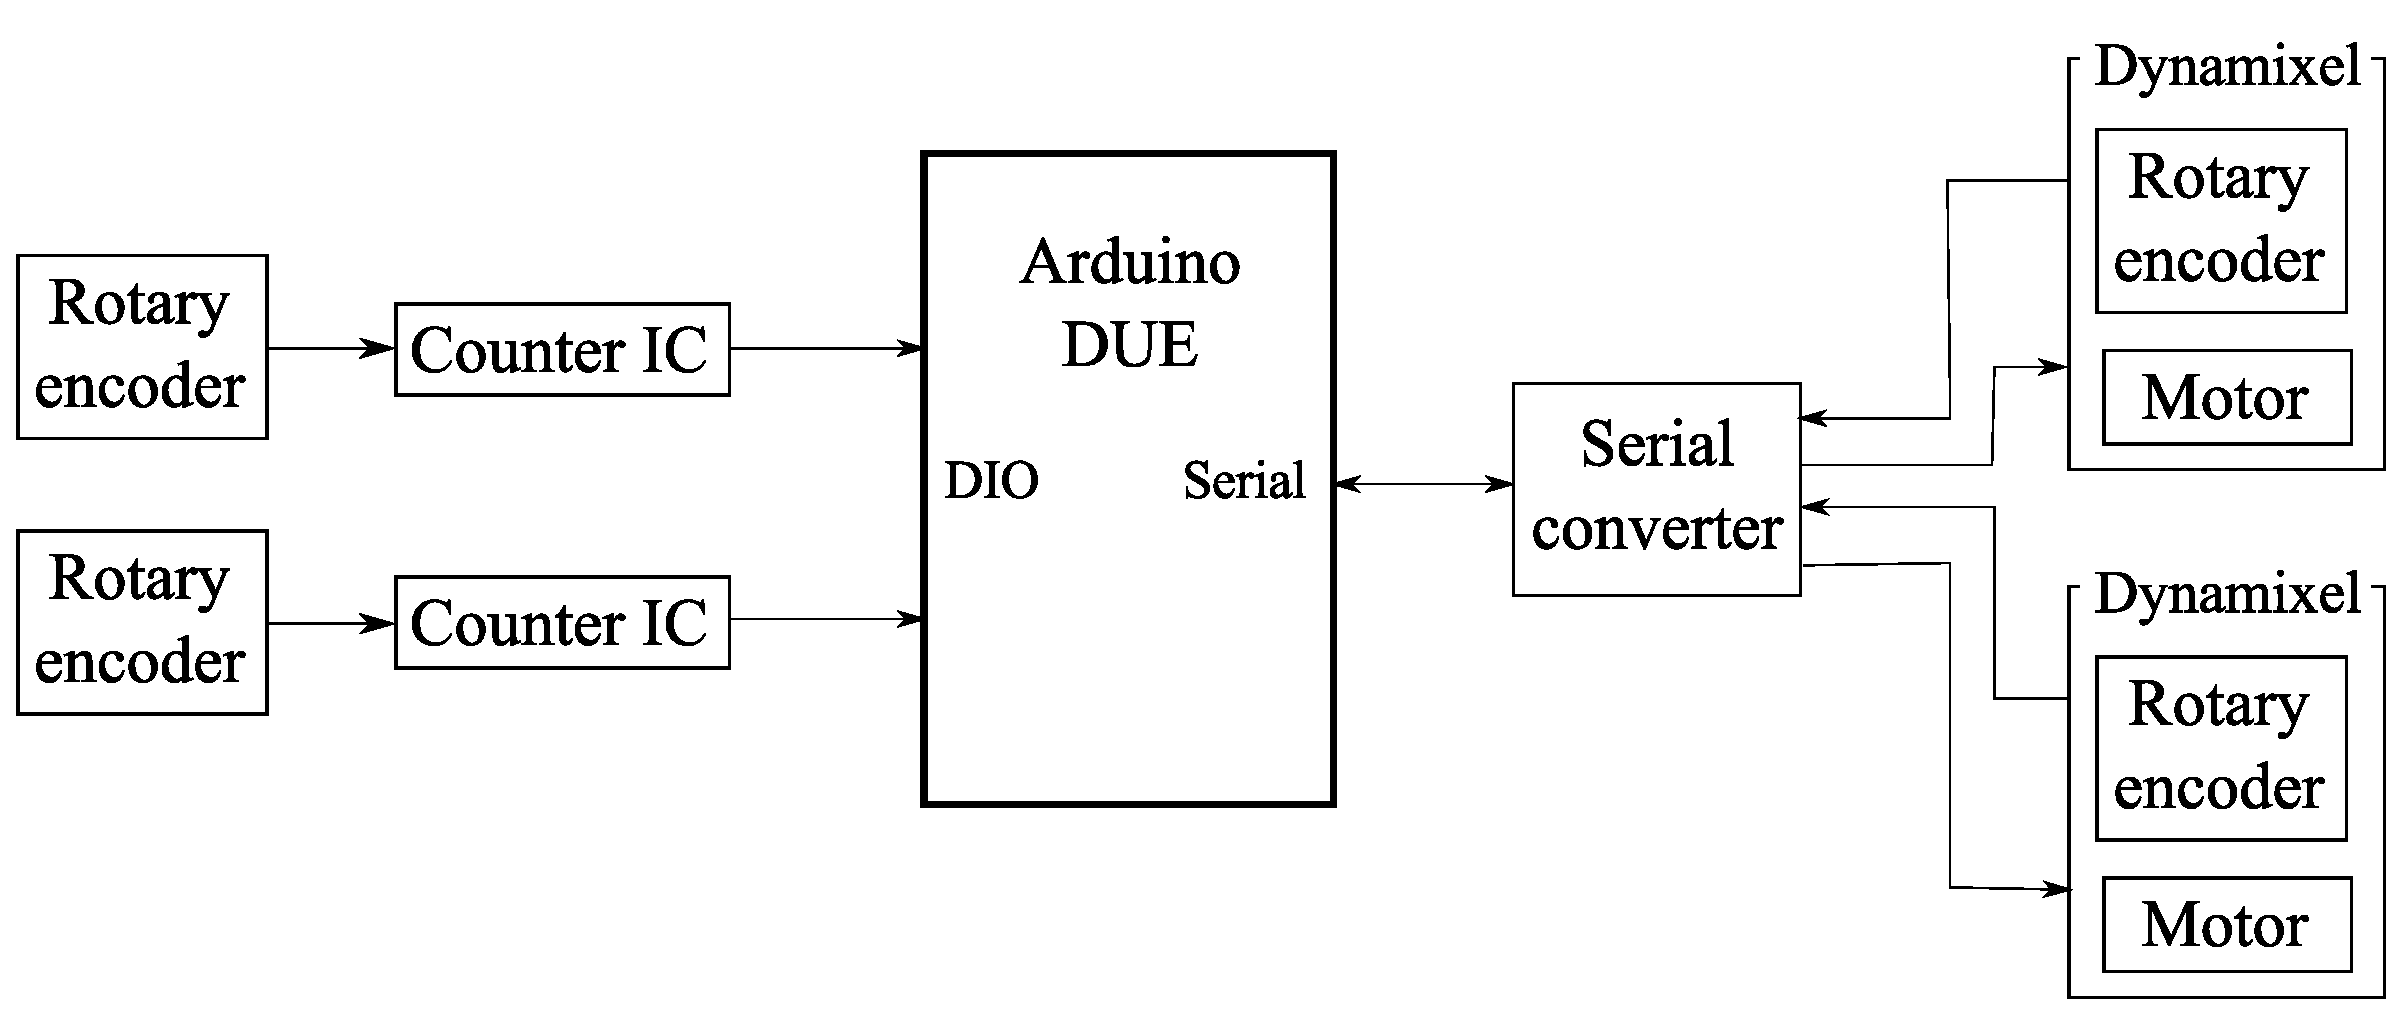
\includegraphics[width=.90\textwidth]{./figure/system.pdf}
	% 	\caption{Control system for the finger}
	% 	\label{fig:system}
	% \end{figure}
	\begin{figure}[tb]
		\centering
		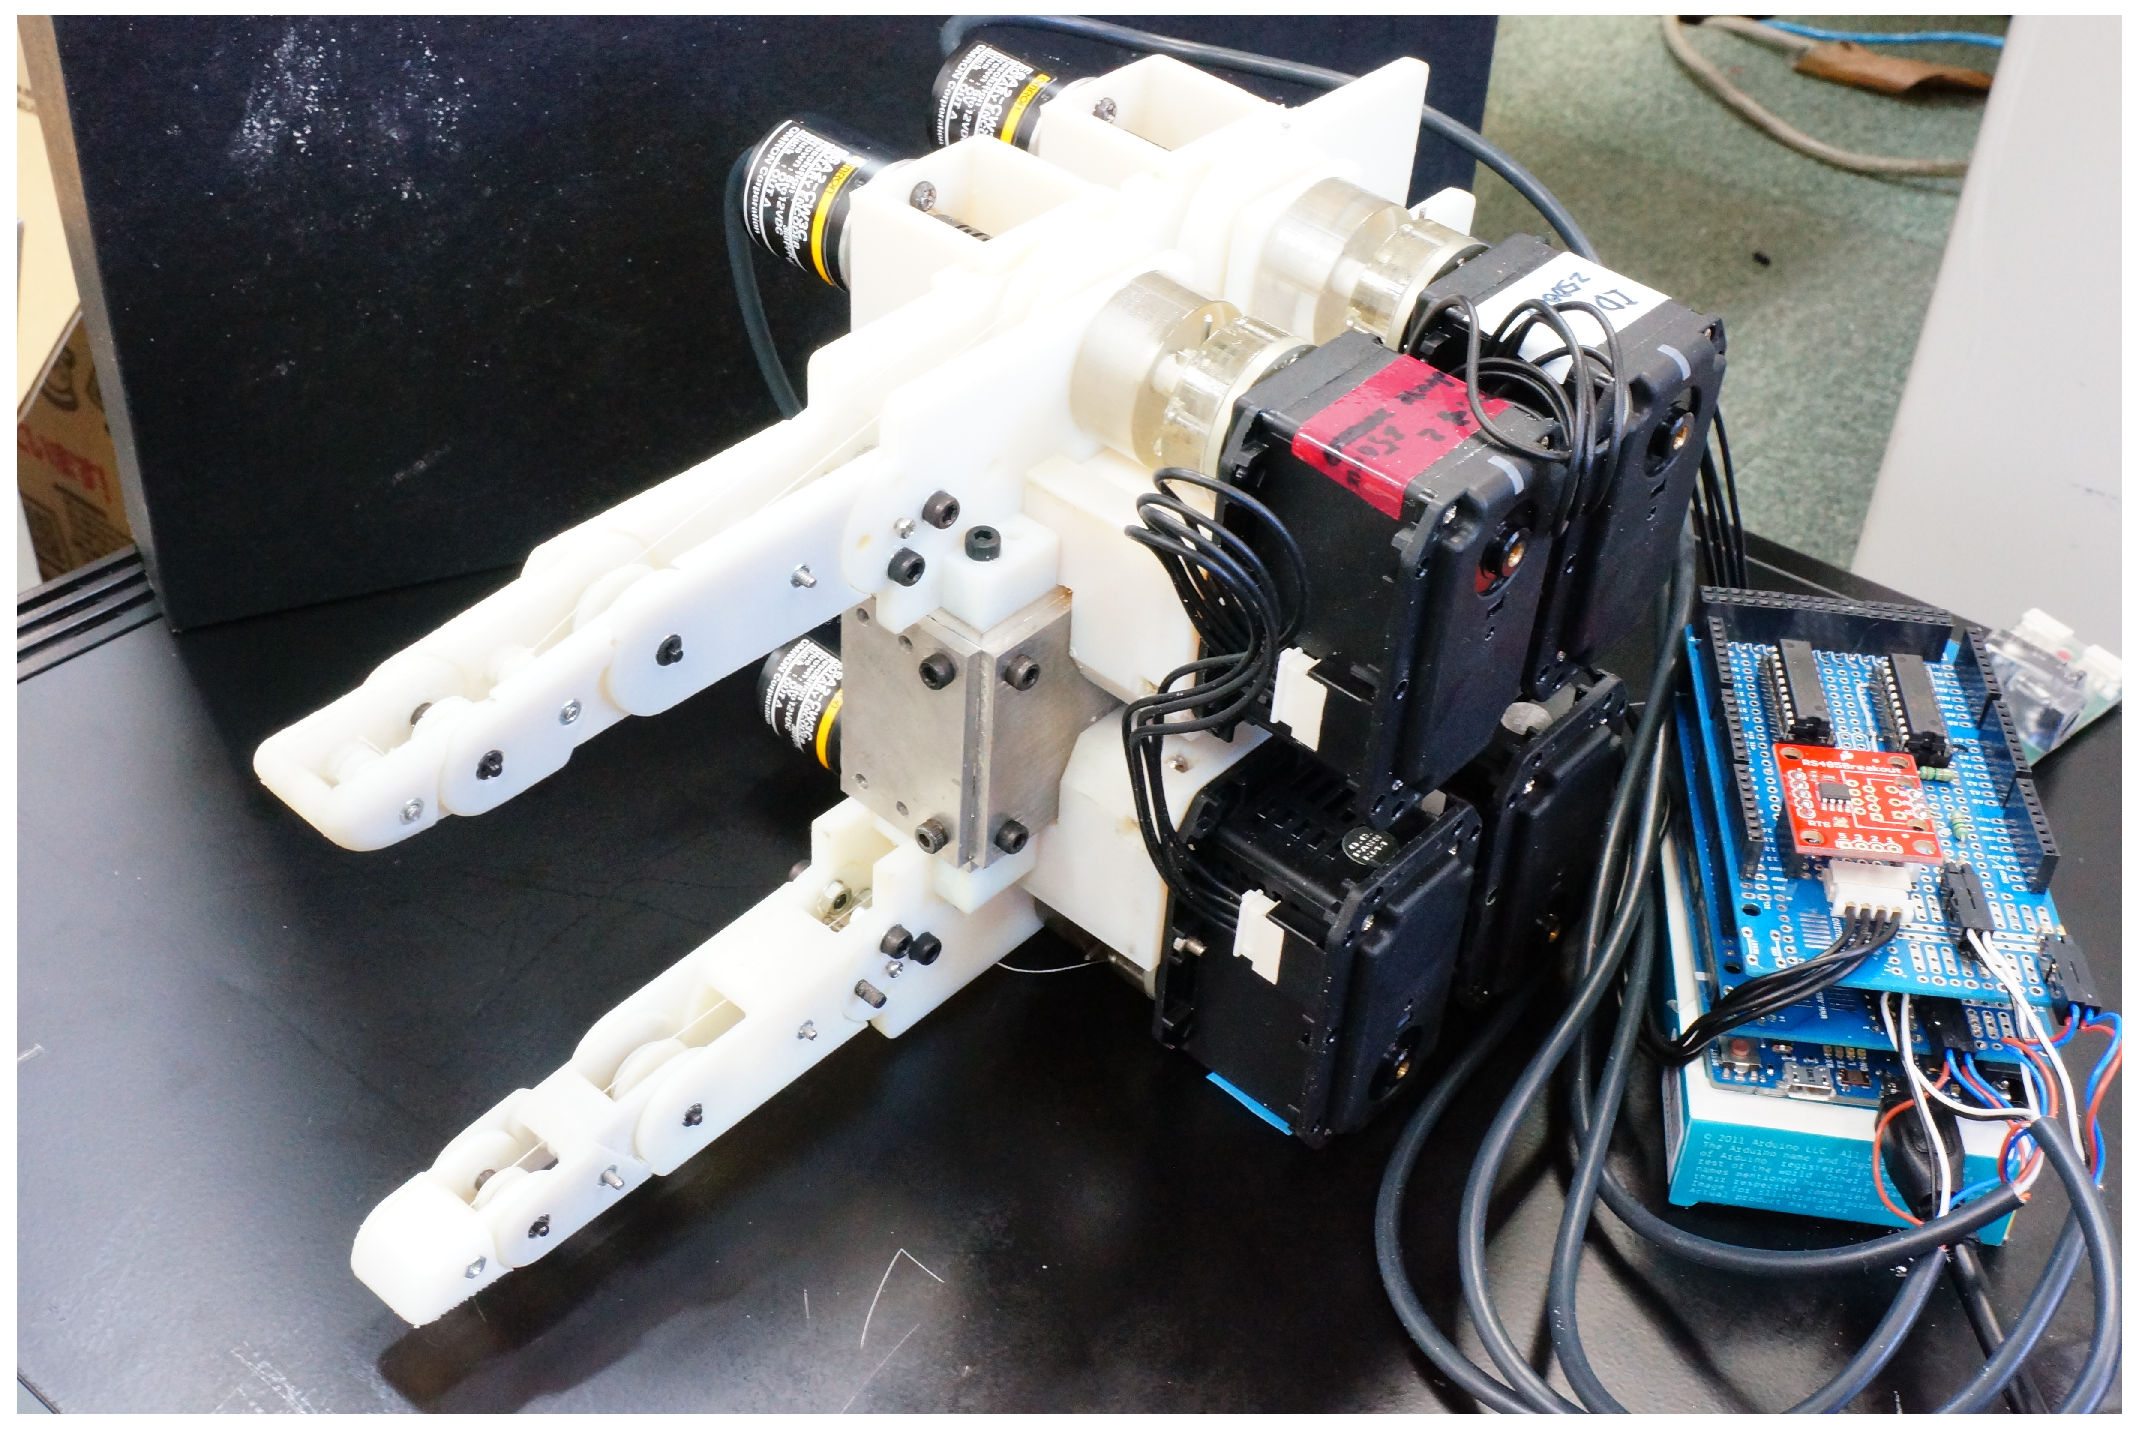
\includegraphics[width=.50\textwidth]{./figure/JPG/finger1.eps}
		\caption{Photograph of the robot hand composed of two underactuated fingers with a branching tendon}
		\label{pic:finger}
	\end{figure}
Each tendon is driven by a servo motor(Dynamixel MX-64R), and
the rotation angle of the base pulley that winds the tendon is measured by rotary encoders (OMRON E6A2-CW3C).
This angle is used to calculate the tendon displacement.
% Tendon displacement can be calculated by this angle.
Pulses from the encoder are counted by an IC counter (NEC $\mu$PD 4702C).
The finger is controlled by Arduino DUE.
Arduino - a microcontroller board that reads the values of the counter from digital input ports
and outputs the commands to the motors by a serial port.
% 		フィンガには,腱を駆動するためのサーボモータと,腱の移動距離を測定するためのロータリエンコーダを,それぞれの腱に1個ずつ,計2個使用している.
% 		また,ロータリエンコーダの出力パルスをカウントするカウンタICを,エンコーダ1つにつき,1つずつ用いている.
% 		フィンガの制御に関する演算と,カウンタの読み取り,モータへの指令は,すべてマイコンボードのArduino DUEで行っている.
% 		各部品について,表\ref{tab:component}にまとめる.

% 		\begin{table}[htbp]
% 		 \centering
% 		 \caption{フィンガに搭載されているパーツ}
% 		 \label{tab:component}
% 		 \begin{tabular}{|c|c|c|}
% 		  \hline
% 		  & 型番 & 備考 \\ \hline \hline
% 		  マイコンボード & Arduino DUE & 32ビットマイコン搭載ボード,動作周波数84MHz \\ \hline
% 		  サーボモータ & Dynamixel MX-64 & 4096ビット角度センサ搭載 \\ \hline
% 		  ロータリエンコーダ & OMRON E6A2-CW3C & インクリメンタル方式,2相,360P/R \\ \hline
% 		  カウンタIC & NEC $\mu$PD4702C & 8ビット・アップ・ダウン・カウンタ \\ \hline
% 		 \end{tabular}
% 		\end{table}

The tensile force $\bm{f}$ and tendon displacement velocity $\dot{\bm{l}}$ are controlled by a winding tendon wire by the base pulley.
The base pulleys are not directly connected to the servo motors, but are driven by linear-torsion springs placed between the servo motors and base pulleys.
The torque exerted by the spring
is calculated from
% can be calculated by subtracting 
the displacement difference between the base pulley and the spring;
therefore, to control the tensile force on the tendon, we must control the spring displacement.
The spiring constant of the selected springs is
% We adopted springs whose spring constant is 
5.17N/mm.
% 		腱駆動のフィンガは,腱の巻き取り量を調整することで,腱張力や腱の移動速度を制御する.
% 		開発したフィンガにおいては,腱に発生する張力を制御するため,腱をモータで直接巻き取るのではなく,ねじりばねを用いることで,力を伝達している.
% 		具体的には,腱を駆動するプーリと,モータの間にねじりばねをはさみ(図\ref{fig:spring}),モータを位置制御することでプーリに発生するトルクを制御する.
% 		ばねに発生しているトルクは,プーリとモータの位置から求まるばねの変位によって計算することができ,このトルクが目標トルクに達するように制御を行う.
% 		今回使用したばねは,ばね定数5.17[N mm/deg],許容変位値30[deg]である.
The displacement angle of base pulley is measured by a rotary encoder directly connected to the shaft of the pully.
% A rotary encoder which measures angle of base pulley is directly connected to a shaft of the pulley.
% 		ロータリエンコーダの取り付けは,簡単のため,駆動軸と直結することにした(図\ref{fig:spring2}).
% 		開発したフィンガでは,駆動軸が高速に回転することはなく,ラジアル方向,スラスト方向ともに,軸に大きな力がかかることはないと判断した.

% 		\begin{figure}[tb]
% 		 \centering
% 		 \subfigure[ねじりばね\label{fig:spring1}]{\includegraphics*[width=.45\textwidth]{./figure/JPG/spring1.eps}}
% 		 \subfigure[駆動軸周り\label{fig:spring2}]{\includegraphics*[width=.45\textwidth]{./figure/JPG/spring2.eps}}
% 		 \caption{駆動部分}
% 		 \label{fig:spring}
% 		\end{figure}

The angular position and fingertip force can be controlled while the tendons do not slacken.
% Fig. \ref{fig:control} shows a position controller for the each motor.
% % 		フィンガは,分岐腱に緩みがないとき,位置制御,もしくは指先に発生する力の制御を行える.
% % 		位置制御するときは,図\ref{fig:control}に示すように制御を行う.
% 	\begin{figure}[tb]
% 		\centering
% 		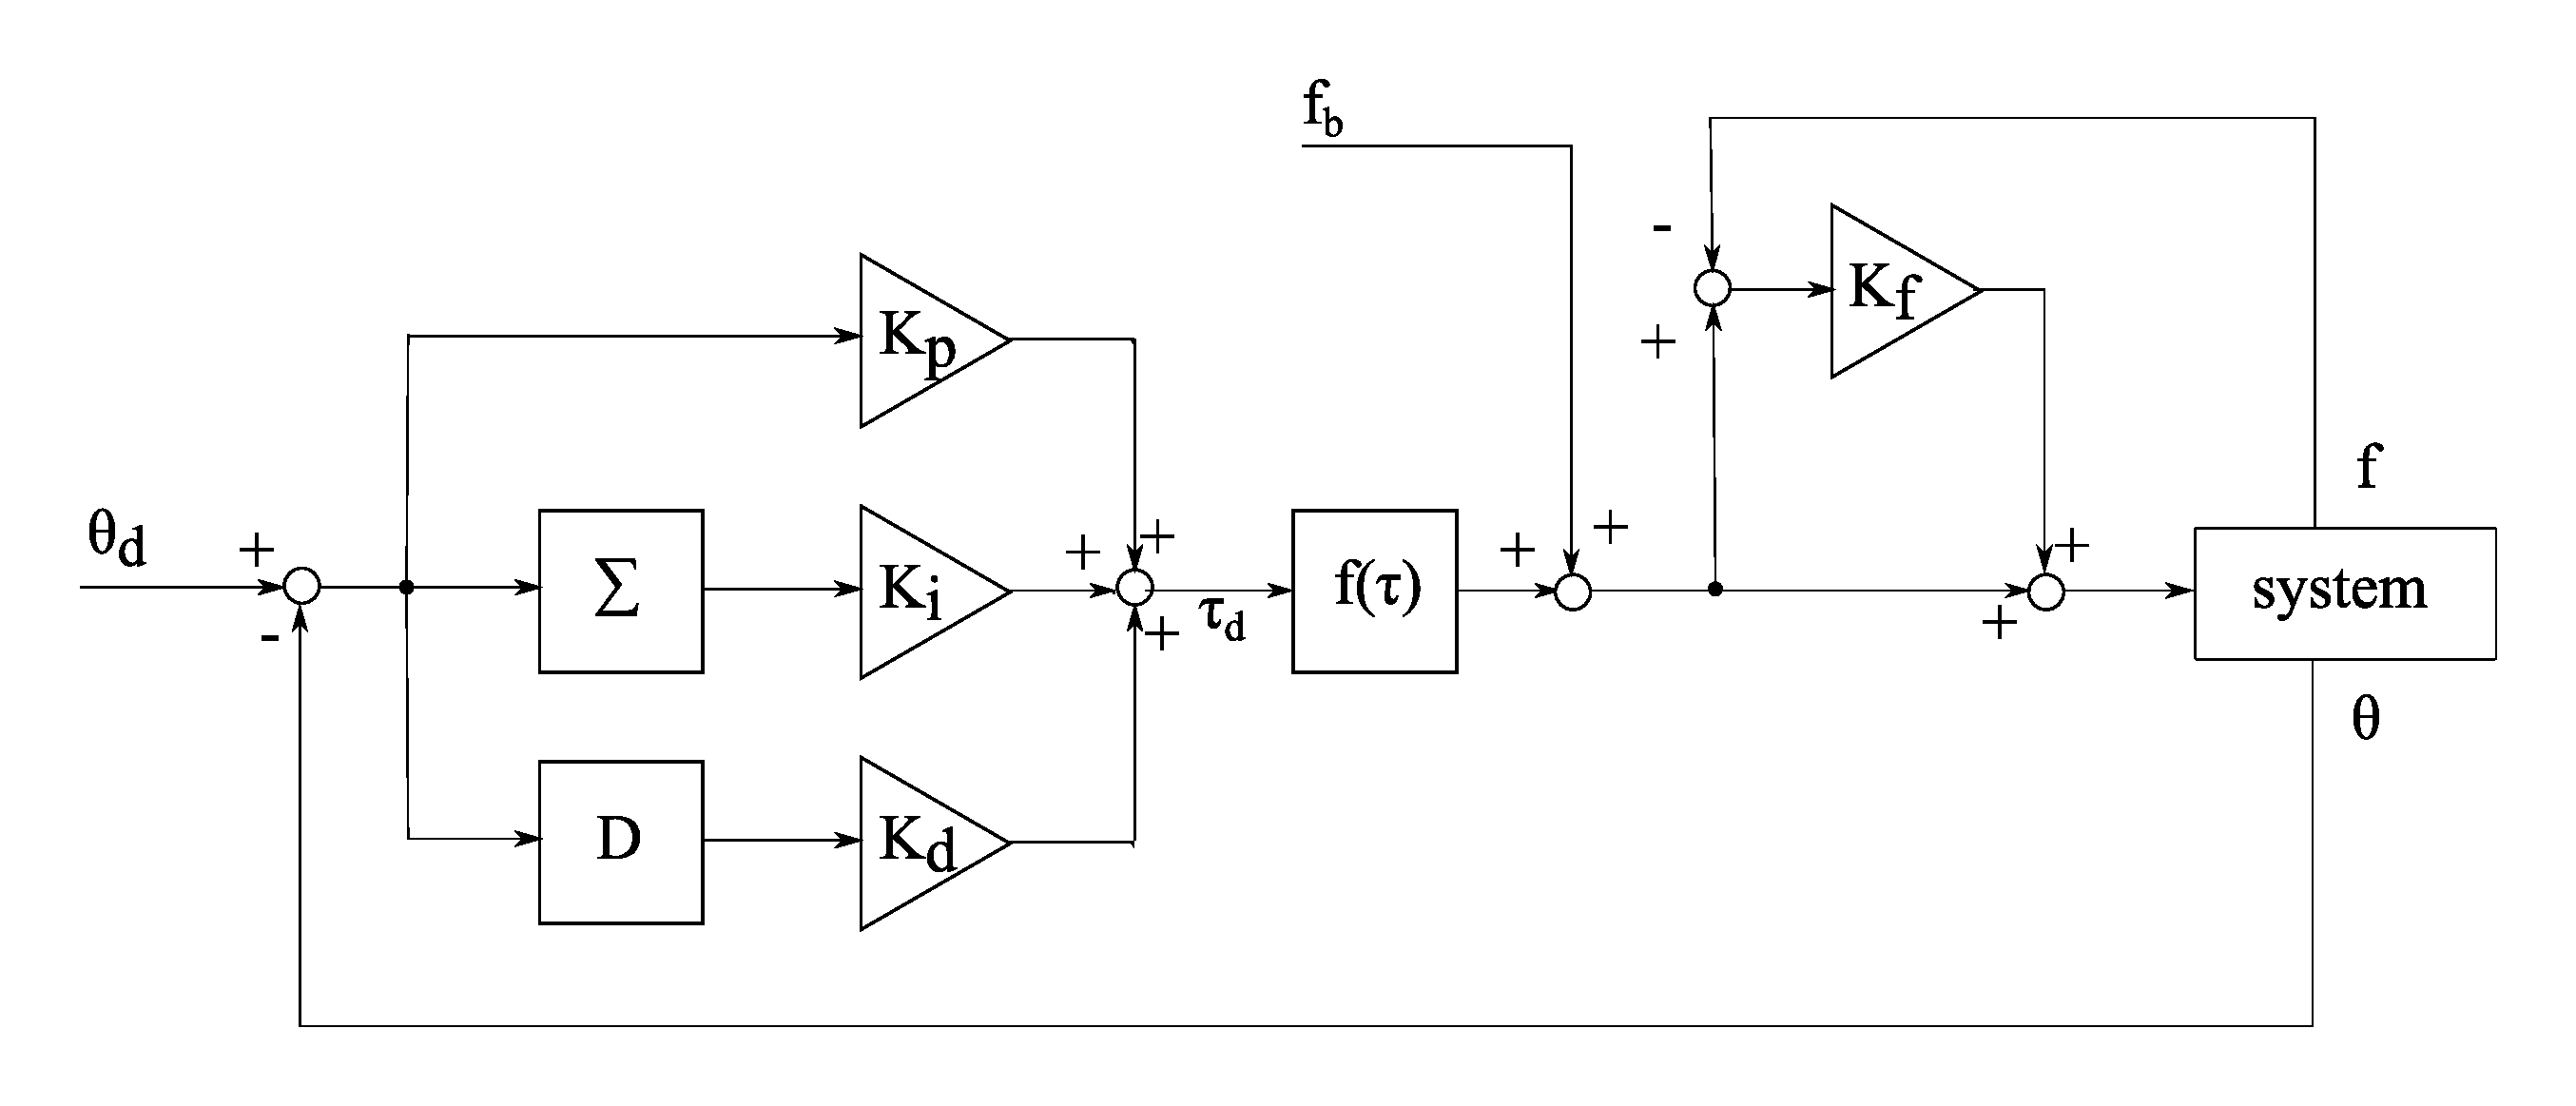
\includegraphics[width=\textwidth]{./figure/control.pdf}
% 		\caption{PID contoller for each motor. D denotes differentiator and S denotes integrator}
% 		\label{fig:control}
% 	\end{figure}
The control is discretized, and the calculation algorithm is iterated by the micro-computer installed on Arduino.
 % repeats the chain of calculation.
% In figure, D reveals differentiator and S is integrator.
% 		この制御は,離散システムであり,マイコンでこの一連の計算を繰り返し行っている.
% 		図中の$D$は微分器を,$\Sigma$は積分器を表す.
The angular position control uses a PID, which calculates the desired spring torque from the position error of a joint.
The current torque of the spring is fed back to the target torque.
% In addition, 
To realize the target torque, a bias force is added to the tendon tensile force.
Because the finger movement is restricted to the horizontal plane, gravity compensation is not included in the system.
% 		位置制御は,目標値とのずれに対してPID制御を行っている.
% 		また,PID制御の結果の目標トルクに対して,実際に駆動軸に発生しているトルクとのずれをフィードバックしている.
% 		フィンガは,水平面内で動作することとし,重力補償は行っていない.
When not needing position control, the finger can move sorely by the feedback control of the spring torque.
The resulting joint torque exerts target forces on the fingertip.
% giving the value of joint torque which exerts target fingertip forces.
% 		物体に接触させて,力をかけるときなど,位置制御を行わないときは,指先に出したい力を発生させる関節トルクを指令値として与え,関節トルクのフィードバックのみで制御を行う.

% bias forceについて説明あった方がいいかも?

Fig. \ref{fig:angle_tracking} plots the tracking performance of the developed system.
% 		以上のようなシステムでフィンガを動作させる.
% 		実際に,関節1の角度が0度の位置から40度の位置まで位置制御を行ったときの,目標角度値に対する,腱の変位から計算される関節1の角度のグラフを図\ref{fig:angle_tracking}に示す.
% 		また,関節1の角度が0度の位置から40度の位置まで位置制御を行ったときの,フィンガの動きを図\ref{pic:angle_tracking}に示す.
\begin{figure}[tb]
	\centering
	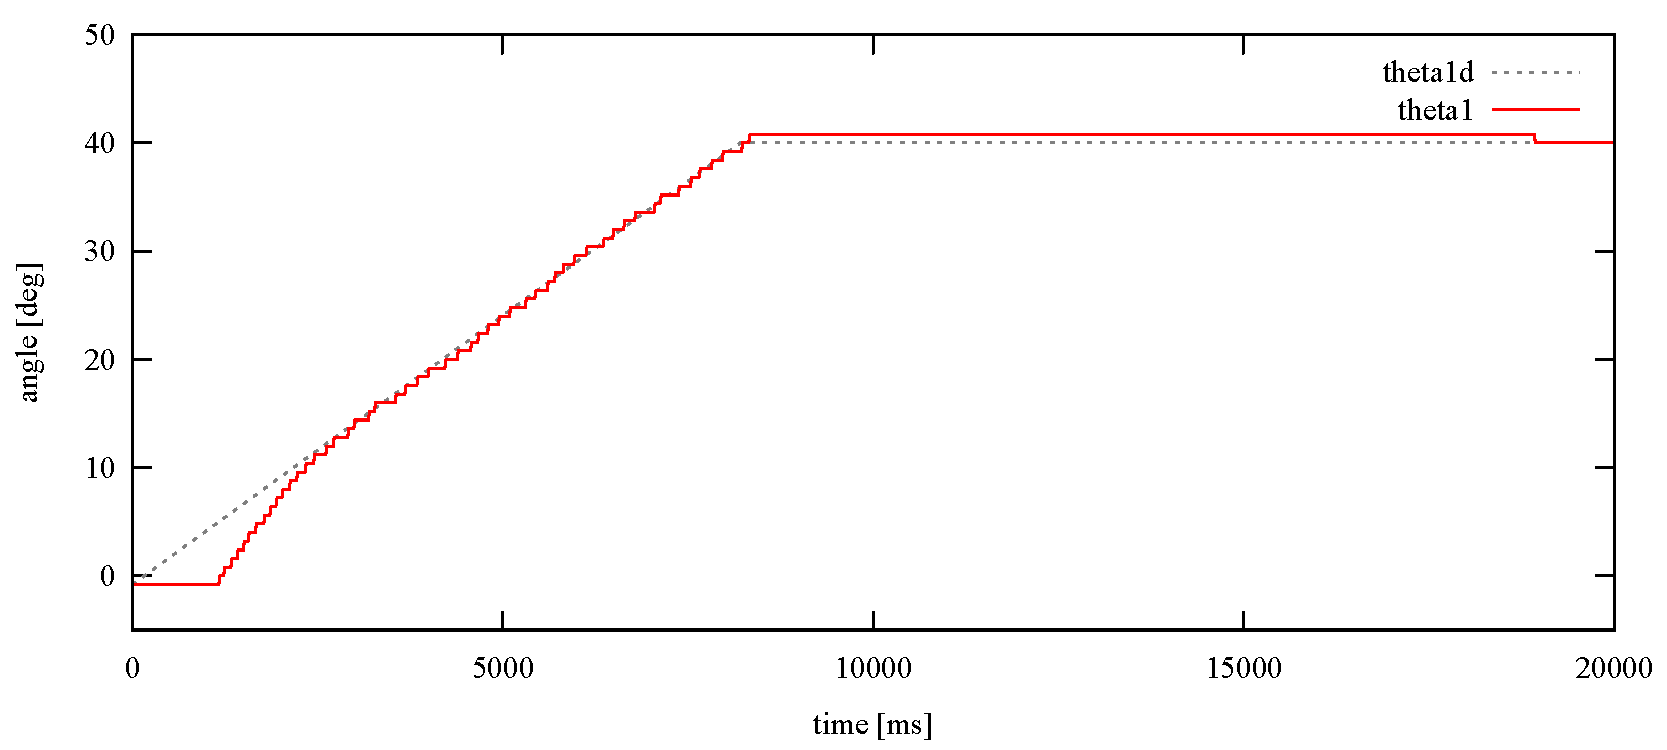
\includegraphics[width=.70\textwidth]{./figure/plot/0208_3_0-20.pdf}
	% \subfigure[0度から40度への移動\label{fig:angle}]{\includegraphics*[width=.90\textwidth]{./figure/plot/0208_3_0-20.pdf}}\\
	% \subfigure[40度から20度への移動\label{fig:angle2}]{\includegraphics*[width=.90\textwidth]{./figure/plot/0208_4_20-10.pdf}}\\
	\caption{Time response of joint angle 1 when the target is a ramp input. Desired angle changes from $0^{\circ}$-$40^{\circ}$ in approximately 8 s. Note the small time delay.}
	\label{fig:angle_tracking}
\end{figure}
% 		\begin{figure}[tbh]
% 		 \centering
% 		 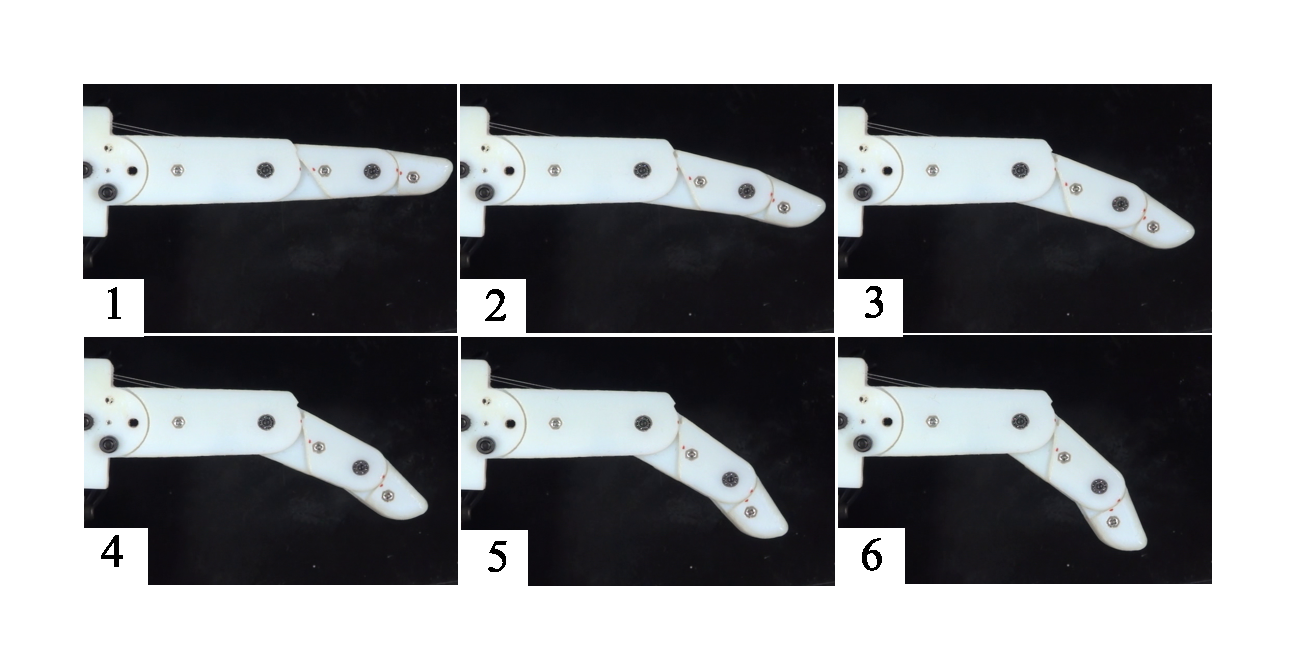
\includegraphics[width=\textwidth]{./figure/frame0208.pdf}
% 		 \caption{位置制御時のフィンガの動き}
% 		 \label{pic:angle_tracking}
% 		\end{figure}
% Table  shows Gain constant when position controling.
% 		このときの位置制御における各ゲインは,表\ref{tab:gain}の通りである.
% 		\begin{table}[htbp]
% 		 \centering
% 		 \caption{位置制御におけるゲイン}
% 		 \label{tab:gain}
% 		 \begin{tabular}{|c|c|}
% 		  \hline
% 		  $K_p$ & 0.05\\ \hline
% 		  $K_i$ & 0.01\\ \hline
% 		  $K_d$ & 0.001\\ \hline
% 		  $K_f$ & 0.1\\ \hline
% 		 \end{tabular}
% 		\end{table}
% We can see delay of i
The initial response is delayed, possibely becasue
% This may be caused by 
rotational friction
% of joints on not the shaft but
is exerted on the surface of the finger frame.
% Though shafts of joints have ball bearing, 
% not shaft but 
At this stage, the gain constants are not optimally configured because position control is not the main focus of our research.
% In this time, we didn't sufficiently configure each gain constant because position control is not main focus in this research.
The gains could be reconfigured in an improved design.
% 
% If we had to improve responsibility, we can configure gain.
% 		グラフからは,フィンガの初動が遅れていることが読み取れる.
% 		これは,関節の回転方向に生じる摩擦力が大きいためだと考えられる.
% 		フィンガの関節には,ボールベアリングが入っており回転軸における摩擦は十分に小さい.
% 		しかし,関節において,フィンガの外装同士が干渉していることが考えられる.
% 		% しかし,軸が,地面と平行になった状態で動作させているため,関節において,.
% 		これを防止する十分なクリアランスが設定できていなかったため,摩擦が大きくなってしまっていると考えられる.

% 		また,目標値への角度の収束が十分に早いとは言えない.
% 		さらに,目標角度が一定のときの外乱に対しても,すぐに抵抗する力が弱く,目標角度への移動にはかなり時間がかかる.
% 		今回は,動作確認のために位置制御を行ったので,PID制御におけるゲインを十分に調整していなかった.
% 		しっかりとゲイン調整を行えば,時間に対する応答性は良くなることが予想される.
		
% 		% (位置制御時の腱張力の割合,それにともなう動きなどについて追加する.また,ヤコビアンの値から,仮想自由度での制御に用いている式を示しておく?)
% 		% subsection control (end)

% 		% section producing (end)

%  \section{開発したフィンガによるグリッパ} % (fold)
%  \label{sec:gripper}
% 	開発したフィンガを2本組み合わせることで,グリッパとして利用することができると考えられる.
% 	その外観は,図\ref{pic:finger}に示した通りである.
% 	グリッパとしての動きのイメージを図\ref{fig:gripper}に示す.
% 	まず,物体に接触するまでは,図\ref{fig:gripper_coupled}に示すように,関節が連動した状態で動かす.
% 	このとき,関節は連動しているので,1自由度のグリッパのように,物体に決まった軌道でアプローチすることになる.
% 	この状態から,バイアス張力を減らしていく,もしくは,指先の力を強めていくと,図\ref{fig:gripper_uncoupled1}のように腱が緩み,形態が変化するようなグリッパとして用いることができるのではないかと考えられる.

% 	\begin{figure}[tb]
% 	 \centering
% 	 \subfigure[連動している状態\label{fig:gripper_coupled}]{\includegraphics*[width=.48\textwidth]{./figure/gripper.pdf}}
% 	 \subfigure[腱1sが緩んだ状態\label{fig:gripper_uncoupled1}]{\includegraphics*[width=.48\textwidth]{./figure/gripperuncoupled1.pdf}}
% 	 \caption{2関節フィンガによるグリッパの模式図}
% 	 \label{fig:gripper}
% 	\end{figure}

% section control_system (end)

% section producing (end)

\section{Validation of Tendon Slack} % (fold)
\label{sec:verification}
% \chapter{2関節フィンガにおける分岐腱の緩み条件の検証} % (fold)
% \label{cha:verification}
Depending on the bias tensile force of tendons and the force exerted on the fingertip,
one of the branched tendons may slacken.
The slacking conditions were described in Section 2.
% We derived the slacking condition in Chapter 2.
This section validates the mechanism in the real environment.
% In this chapter, we will validate it in the real environment.
% 	\ref{sub:tendon_slack}項で述べたように,開発したロボットフィンガでは,フィンガが指先に発生する力と腱のバイアス張力の条件によって,腱に緩みが生じる.
% 	計算により求めたこの条件が,実際の状況に即しているかどうか,実機により検証を行った.
% 	本章では,検証実験の手順と結果について述べる.

% 	\section{緩み条件検証の手順} % (fold)
% 	\label{sec:slack_experiment}
% 		\ref{sub:tendon_slack}項で計算されたように,分岐腱の緩み条件は,フィンガの角度や指先の力によって決まる.
% 		ここでは,開発したフィンガにおける緩み条件の具体的な値と,実験の手順について述べる.
% 		\subsection{フィンガにおける緩み条件} % (fold)
% 		\label{sub:valiables_of_slack}

The tendon slackens when the tensile force of tendn 2a or tendon 2b in (\ref{eq:f-tau-pinv}) becomes zero.
% When tensile force of tendon 2a or that of 2b in (\ref{eq:f-tau-pinv}) is zero, the tendon slacks.
Substituting real parameters of the robot hand into (\ref{eq:f-tau-pinv}), we obtain
% 			腱が緩む条件は,式(\ref{eq:slack-f})で計算される腱張力ベクトルの成分のうち,腱1p,1sの腱張力どちらかが負になることである.
% 			本研究で開発したフィンガにおいて,腱ヤコビアン$\bm{J}$は式(\ref{eq:J_value})のように与えられるので,これを用いて,式(\ref{eq:f-tau-pinv})における$\bm{A}$,$\bm{f}_b$を計算すると,
% \begin{align}
% 	\bm{A} = \begin{bmatrix}
% 		-0.0606 & -0.0492	\\
% 		-0.0606 & 0.2008	\\
% 		0.1515 & -0.1894
% 	\end{bmatrix},	
% 	\bm{f}_b = \begin{bmatrix}
% 		1 \\
% 		1 \\
% 		0.8
% 	\end{bmatrix}f_b, 
% \end{align}
% 			となる.
% 			ここで,式(\ref{eq:f-tau-pinv})において,$\bm{\xi} = \xi\begin{bmatrix}1 & 1 & 1\end{bmatrix}^T$とし,さらに,$\bm{f}_b$の腱2に対するバイアス張力が$f_b$となるように,係数$\xi$を調整したものを,$f_b$とおいている.
% When coupling of two joints, using $\theta_1=2\theta_2$, $\bm{f}$ is described from (\ref{eq:slack-f}) as follows:
% 			これより,式(\ref{eq:slack-f})において,$\bm{f}$を求めると,
% 			\begin{align}
% 				\bm{f} = \begin{bmatrix}
% 					f_2		\\
% 					f_{1p}	\\
% 					f_{1s}
% 				\end{bmatrix} = \begin{bmatrix}
% 					0.0606L_1\cos\theta_1+0.1098L_2\cos(\theta_1+\theta_2)	\\
% 					0.0606L_1\cos\theta_1-0.1402L_2\cos(\theta_1+\theta_2)	\\
% 					-0.1515L_1\cos\theta_1+0.0387L_2\cos(\theta_1+\theta_2)
% 				\end{bmatrix}s
% 				+\begin{bmatrix}
% 					1 \\
% 					1 \\
% 					0.8
% 				\end{bmatrix}f_b,
% 			\end{align}
% 			となる.
% 			さらに,関節が連動しているとき,$\theta_1 = 2\theta_2$なので,
\begin{align}
	\begin{bmatrix}
		f_1		\\
		f_{2b}	\\
		f_{2a}
	\end{bmatrix} = \begin{bmatrix}
		0.0606L_1\cos2\theta_2+0.1098L_2\cos3\theta_2	\\
		0.0606L_1\cos2\theta_2-0.1402L_2\cos3\theta_2	\\
		-0.1515L_1\cos2\theta_2+0.0387L_2\cos3\theta_2
	\end{bmatrix}F
	+\begin{bmatrix}
		1 \\
		1 \\
		0.8
	\end{bmatrix}f_b,\label{eq:independent-f}
\end{align}
where $f_b$ is the bias tensile force variable.
From (\ref{eq:independent-f}), we can derive the $f_b$ that renders either $f_{2a}$ or $f_{2b}$ zero, as a function of $F$ and $\theta_2$.
Fig. \ref{fig:slack} shows the bias force $f_b$ that retains $f_{2a}$ and $f_{2b}$ positive.

% $f_b$ can be described ...
% 			となる.
% 			ここで,腱張力が負にならないように調整できる変数は3つ存在する.
% 			1つは,フィンガが指先に出す物体に対して垂直な方向の力の大きさ$f$である.
% 			2つ目は,物体に接触したときの関節2の角度$\theta_2$である.
% 			最後は,腱のバイアス張力$\bm{f}_b$の大きさである.
% Fig. \ref{fig:slack-angle}...
% 			ここでは,$f$と$\theta_2$をそれぞれ固定したときに,$f_{1p}$,もしくは$f_{1s}$がちょうど$0$になる$f_b$の値を,分岐腱の緩みの条件として考え,図\ref{fig:slack}に示す.
% 			図\ref{fig:slack-angle}は,$f=0.6$としたときの,角度$\theta_2$に対して,$f_{1p}$,$f_{1s}$がちょうど$0$になる$f_b$の値ををれぞれグラフにしたものである.
% 			グラフの横軸は関節2の角度であり,フィンガが最大に伸展している状態の$\theta_2=0^{\circ}$から,フィンガの指先が物体に対して垂直になる,$\theta_2=30^{\circ}$までを範囲としている.
% 			図\ref{fig:slack-force}は,$\theta_2=15^{\circ}$としたときの,$s$に対して,$f_{1p}$,$f_{1s}$がちょうど$0$になる$f_b$の値ををれぞれグラフにしたものである.
% 			グラフの横軸は,フィンガが指先に発生させる力であり,フィンガに使用したねじりばねの最大トルクを考慮して$s=2$までを範囲としている.
\begin{figure}[tbhp]
	\centering
	\subfigure[Limit of $f_b$ versus $\theta_2$ when $F=0.6$\label{fig:slack-angle}]{\includegraphics*[width=.49\textwidth]{./figure/plot/threshold_angle.pdf}}
	\subfigure[Limit of $f_b$ versus $F$ when $\theta_2=15^{\circ}$\label{fig:slack-force}]{\includegraphics*[width=.49\textwidth]{./figure/plot/threshold_force.pdf}}
	\caption{Limiting values of $f_b$ at which $f_{2a}$ or $f_{2b}$ remains positive}
	\label{fig:slack}
\end{figure}
% 			ここで,開発したフィンガの指先に追加パーツをつけたため,$L_1=30.5,L_2=37.5$として計算した.
As shown in that figure, on the developed finger, the $f_b$ at which $f_{2a}$ vanishes is larger than that of $f_{2b}$, at any $\theta_2$ and $F$.
Therefore, $f_{2a}$ falls to zero and tendon 2a loosens while $f_{2b}$ is stil positive and $f_b$ gradually declines.
% 			グラフに示した値を下回る$f_b$をバイアス張力としてかけてフィンガを動作させると,対応する腱の張力は負になるため,腱が緩む.
% 			グラフから分かるように,開発したフィンガでは,グラフに示されている範囲において,いかなる$\theta_2$,$s$の値においても,腱1pよりも腱1sの方が,張力が0になる$f_b$の値が大きい.
% 			したがって,$f_b$を十分に大きい値から徐々に下げていくと,腱1sの張力が先に0となり,腱が緩むことになる.
To slacken tendon 2b, we must change the moment arms that define the values of the matrix $\bm{P}$.
% In order to make tendon 2b slack, we have to change moment arms which defined the values of the matrix $\bm{P}$.
% 			この条件には,計算の過程から分かるように,フィンガの腱ヤコビアンが関係する.
% 			また,腱ヤコビアンの成分は,腱のモーメントアームになっているので,今回開発したフィンガとは違い,腱1pを先に緩ませようと思うと,モーメントアームを変更する必要がある.
% 			このようなモーメントアームの一例としては,表\ref{tab:slack_momentarm}のような組み合わせがある.
% 			\begin{table}
% 				\centering
% 				\caption{異なる緩み状態を実現するモーメントアームの一例}
% 				\label{tab:slack_momentarm}
% 				\begin{tabular}{|c||c|c|c|} \hline
% 					関節 & 腱2 & 腱1p & 腱1s \\ \hline\hline
% 					関節1 & $ r_{p1}$ & $ r_{t1}$ & $ r_{m1}$ \\
% 					 & 15 & 3 & 5 \\ \hline
% 					関節2 & $ r_{p2}$ & $ r_{t2}$ & - \\
% 					 & 1 & 4 & - \\ \hline
% 				\end{tabular}
% 			\end{table}
This change requires new pulleys because the diameter of the joint pullyes decides the moment arms.
% This change need to produce new pulleys because the moment arms represented by the diameter of pulleys on joints.
% 			モーメントアームは,フィンガの関節に組み込まれているプーリによって実現しているため,変更には,新たなプーリを製作する必要がある.
			
% 			今回は,新たなプーリを作り,緩みを再現することはしないが,このように,モーメントアームの変更により,緩む腱を選ぶことができる.

% 		% subsection valiables_of_slack (end)

% 		\subsection{実験方法} % (fold)
% 		\label{sub:process_of_experiment}
The slacking condition (\ref{eq:independent-f}) was validated in an ezperiment.
% We conducted experiments to validate the slacking condition (\ref{eq:independent-f}).
% Fig. \ref{pic:experiment} shows the appearance of experiment.
% 			前節で述べた,開発したフィンガにおける分岐腱の緩み条件が,実際の動きとどの程度一致するか,検証のため実験を行った.
% 			実験の様子を,図\ref{pic:experiment}に示す.
% \begin{figure}[tbhp]
% 	\centering
% 	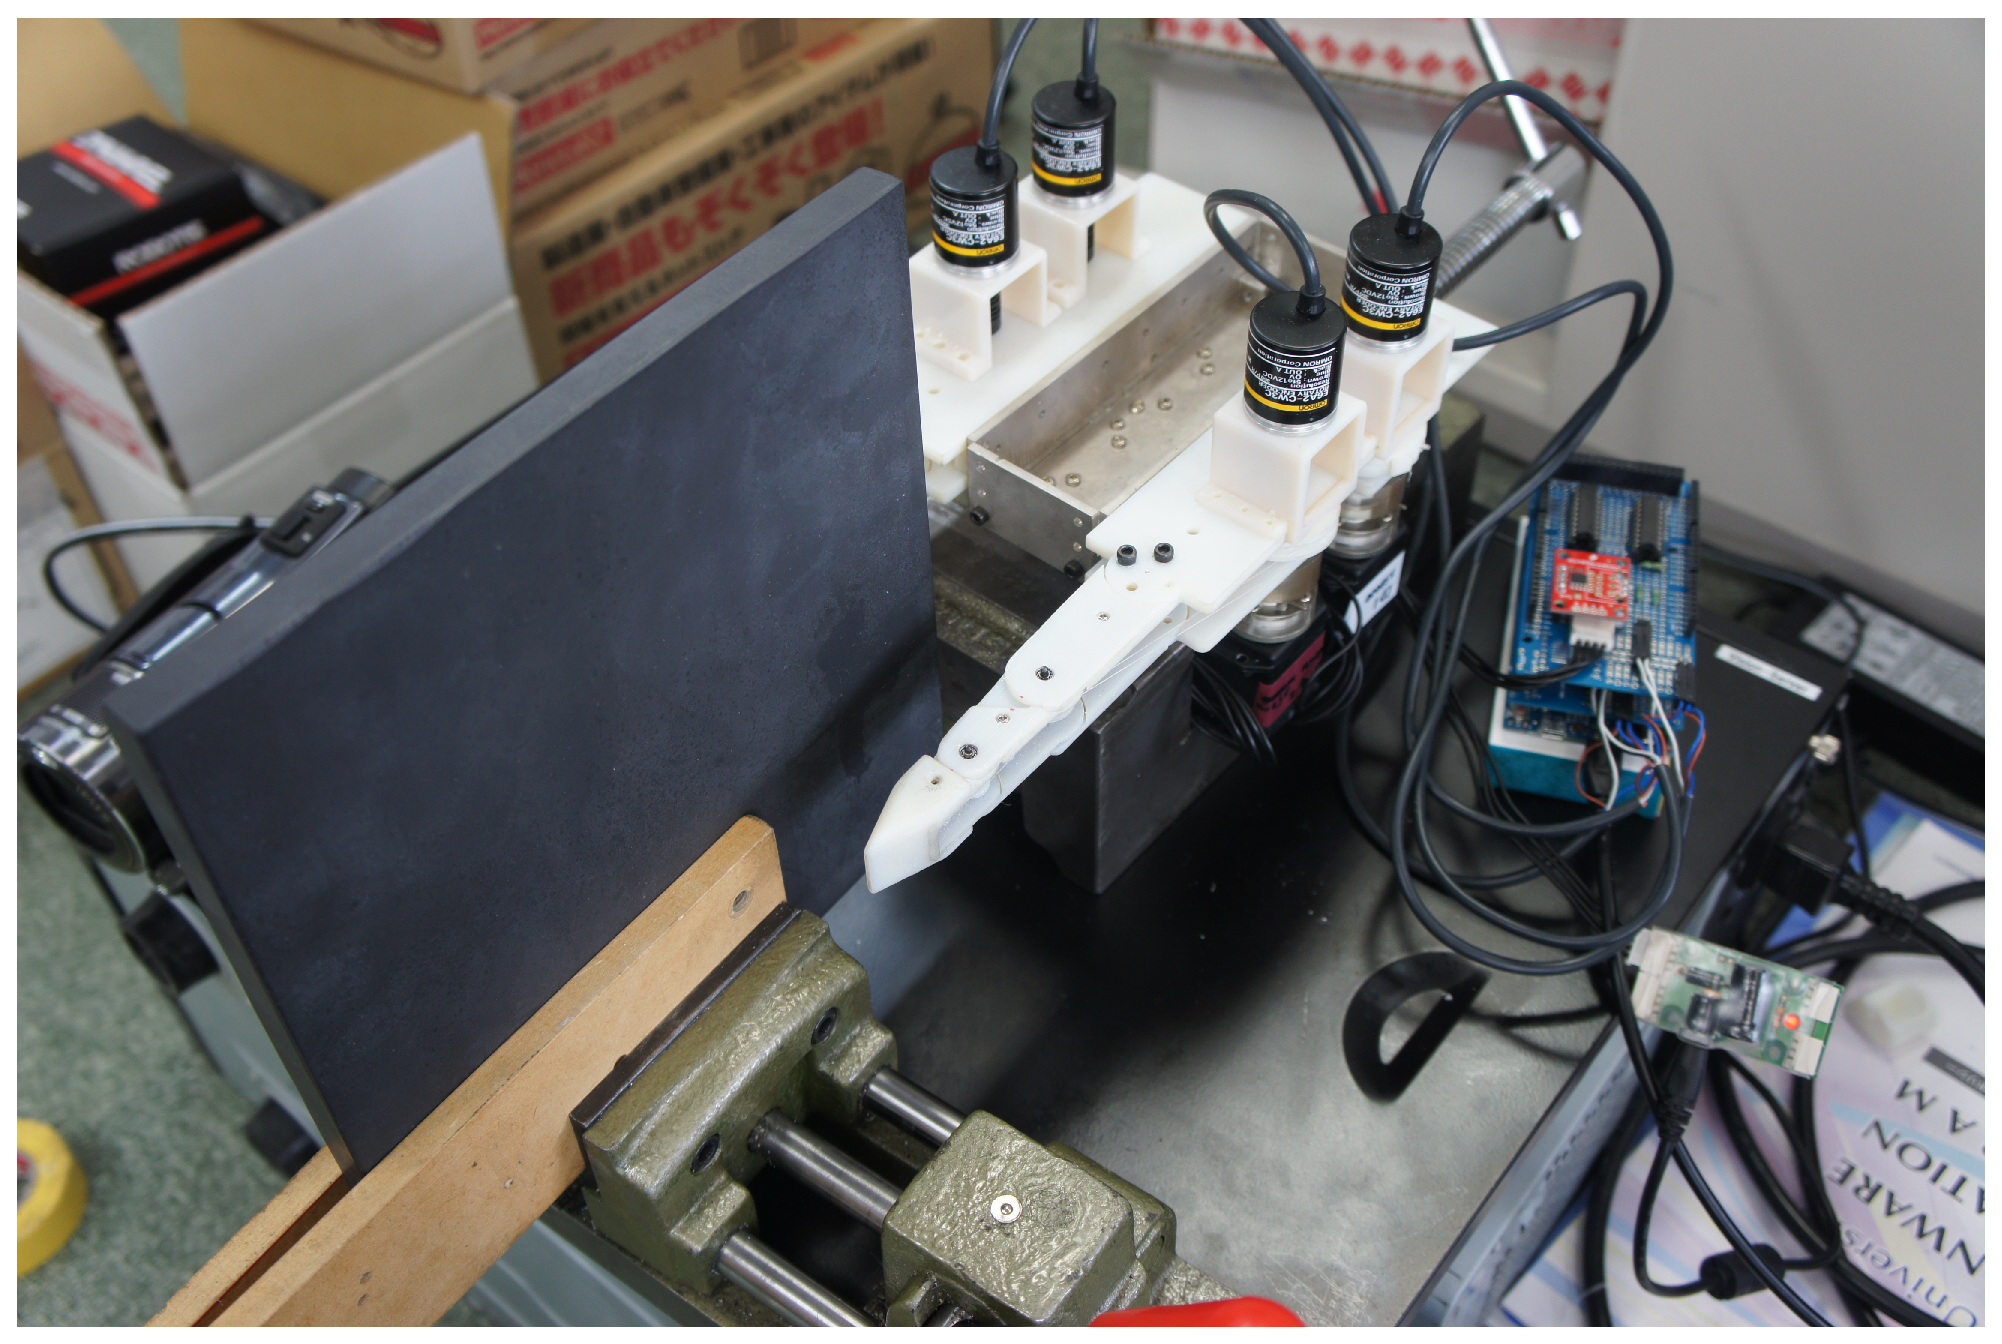
\includegraphics[width=.60\textwidth]{./figure/JPG/experiment2.eps}
% 	\caption{Appearance of experiment}
% 	\label{pic:experiment}
% \end{figure}
% 			実験(1)として,まず,$\theta_2=15^{\circ}$で,$s=0.6, s=0.8$に対して,十分に大きいバイアス張力でフィンガを動作させ始め,バイアス張力を徐々に緩めていき,緩みの条件の値を下回ったときに,分岐腱が緩むことを確認した.
The bias force $f_b$ that loosens the tendon depends on the joint angle and fingertip force
% 			緩み条件は,前述のように,関節の角度と,指先の力に関係して変化するため,実験では,
% 			\begin{itemize}
% 				\item 関節の角度と指先の力を固定し,さまざまなバイアス張力を加えたときのフィンガの挙動を確認した.
% 				\item その後,角度はそのままに,指先の力を変えて同様の実験を行い,指先の力に対する緩み条件の違いを確認した.
% 				\item 最後に,ある大きさの指先の力に対して,関節の角度を変え,フィンガの動きを確認した.
% 			\end{itemize}
, and was experimentally determined by the following steps.
% For experimentally finding $f_b$ to slack a tendon,
% 			実験手順は以下の通りである.
\begin{enumerate}
	\item A large $f_b$ was applied to retain joint coupling,
	\item The finger was actuated to generate a certain fingertip force $F$.
	\item The finger was brought into contact with a low-friction board at a specified angle $\theta_2$ of joint 2.
	\item $f_b$ was gradually decreased until it was sufficiently small to loosen tendon 2a.
\end{enumerate}
% 			\begin{enumerate}
% 				\item 腱張力が0の状態から,バイアス張力をかけ,フィンガを伸びた状態で安定させる.
% 				\item 指先に発生させる力に対応する関節トルクが発生するように,腱に張力をかけ,フィンガを動かす.
% 				\item 所定の角度で指先が接触するように固定した,摩擦の少ない板に指先を当てて,力をかけさせる.
% 				\item バイアス張力を徐々に小さくしていき,腱の緩みを観察する.
% 				\item 腱が緩み,関節の連動が崩れるか,計算された駆動軸のトルクが負になるまで,フィンガを動作させ,元の伸ばした状態に戻す.
% 			\end{enumerate}
Becasue the ratio of the bias force between tendons 1 and 2 is $1:1.8$, 
the bias force cannot generate the joint torques and 
the finger remains stationary.
In practice, however, the finger moves at this ratio
because of the difficulty in zeroing the initial displacement of the torsion spring, and other factors.
% This is caused by various factor such as difficulty to set initial displacement of torsion spring to zero.
Therefore, prior to experiment,
% Then, before starting experiment, 
we stabilized the finger by applying a bias force at the point where the finger extends in a straight line.
Here, the ratio of the bias force is the ratio of the tensile force in tendon 2 to that in tendon 1.
% We use the ratio of tendon 2 tensile force to tendon 1 in this time as the ratio of bias force. 
% 			また,腱2と腱1の間のバイアス張力の比は,計算通りであれば,$1:1.8$になれば関節にトルクは発生せず,フィンガは運動しないはずである.
% 			しかし,実際には,ねじりばねの初期変位を0に設定することの難しさなどの要因から,この比のバイアス張力をかけるとフィンガが運動してしまう.
% 			フィンガの運動において,トルクの発生しない腱張力は重要であるため,理論式とは一致しないが,これは,調整して釣り合いのとれた値を探す必要のある部分である.
% 			そこで,実験を始める前に,$\theta_1,\theta_2=0$になるように位置制御を行い,フィンガが伸びた状態で安定させ,このときの腱2の腱張力を1とした場合の腱1の腱張力を求め,これを前述のバイアス張力の比として利用することとした.
% 			この比は,測り直す度に微妙なずれが生じるため,(1)から(3)の実験中,この比の値は一定とし,実験結果に与える影響に大差がつかないようにした.
% 			ただし,実験(4)は,(3)までと別の日に行ったため,腱張力の比は,同じではない.
% 			しかし,実験の前に,フィンガを安定させて腱張力の比をとる作業を行っている.

% 		% subsection process_of_experiment (end)

% 	% section slack_experiment (end)

% 	\section{結果・考察} % (fold)
% 	\label{sec:slack_conclusion}
The actuation of the finger at joint angle $\theta_2=15^{\circ}$
and fingertip forces $F=0.6$ and $0.8$ is shown in Fig. \ref{fig:slack_conclusion}.
% The result obtained by actuation of finger using $\theta_2=15^{\circ}$ as joint angle 
% and $F=0.6,0.8$ as fingertip force 
% is shown in Fig. \ref{fig:slack_conclusion}.
% In addition, 
An example of finger movement throughout the experiment is shown in Fig. \ref{pic:example_slack}.
% 		まず,関節の角度を$\theta_2=15^{\circ}$,フィンガの出す力を$s=0.6$と$s=0.8$として,十分に大きなバイアス張力でフィンガを動かし始めたときの実験結果を,図\ref{fig:slack_conclusion}に示す.
% 		また,実験時のフィンガの動きの例を図\ref{pic:example_slack}に示す.
	\begin{figure}[tb]
	\centering
		\subfigure[$F=0.6$\label{fig:r60b500}]{\includegraphics*[width=.49\textwidth]{./pdf/2320t15r60b500shadow.pdf}}
		\subfigure[$F=0.8$\label{fig:r80b450}]{\includegraphics*[width=.49\textwidth]{./pdf/2425t15r80b450shadow.pdf}}
		\caption{Result of actuation experiment at $\theta_2=15^{\circ}$}
		\label{fig:slack_conclusion}
	\end{figure}
	\begin{figure}[tb]
		\centering
		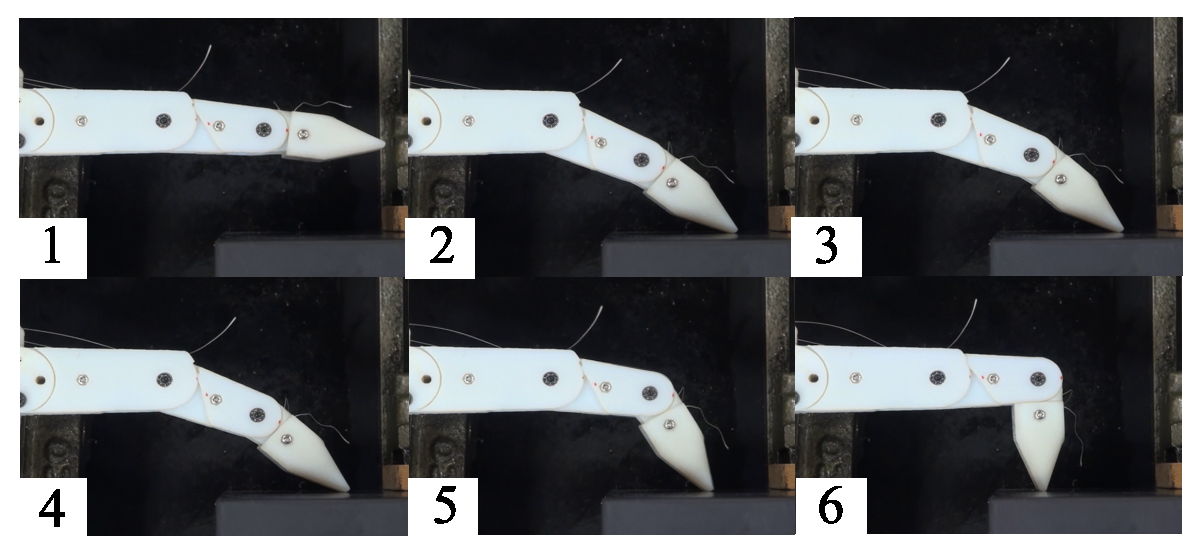
\includegraphics[width=.90\textwidth]{./figure/frame1733r60b180.pdf}
		\caption{Example of finger movement during the experiment. The finger moves when the bias tensile force $f_b$ falls below the limit that retains positive tensile force in tendon 2a.}
		\label{pic:example_slack}
	\end{figure}
In Fig. \ref{fig:slack_conclusion}, the "bias force" is the value of $f_b$ in (\ref{eq:independent-f}), which is also the bias force in tendon 1.
The "encoder angle" is the angle displacement of the drive shaft measured by the rotary encoder that drives tendon 2.
The gray region is the region of negative tensile force in tendon 2a is minus.
% 		グラフは,横軸が時間[ms]で,縦軸は,バイアス張力の大きさ[N]とエンコーダが測定した駆動軸の回転角度[deg]である.
% 		バイアス張力は,式(\ref{eq:independent-f})における$f_b$の値であり,腱2のバイアス張力の大きさに相当する.
% 		エンコーダの角度は,分岐腱である腱1を駆動しているプーリに直結されている,ロータリエンコーダの測定値から計算した,駆動軸の角度変位である.
% 		エンコーダの値は腱1が伸びたとき,つまり,連動状態のフィンガが屈曲方向に動いたときに,増加する.
% 		ここで,グラフでは,バイアス張力が分岐腱の緩む条件となる,下限値thresholdを点線で示し,これを下回っている部分に,グレーの色づけを行っている.
As shown in the graph, tendon 2a becomes slack and the finger movement increases the encoder value as the bias tensile force $f_b$ falls below the limit that retains positive tensile force in tendon 2a.
Thus, we have verified that the slackening of one of the branching tendons is governed by the magnitude of the bias tensile force.
% 		グラフから分かるように,徐々に下げていったバイアス張力$f_b$の値が,腱1sの張力を正に保つことができる下限値を下回ると,腱が緩み,フィンガが動いてエンコーダの値が増加している.
% 		このように,バイアス張力により,分岐腱の緩みを生じさせることができることがわかった.

	
% 		エンコーダによる駆動軸の角度を観測すると,フィンガに大きな動作がない間も,値が徐々に増加していることが観察できる.
% 		この値の増加は,駆動軸が腱が緩む方向に微小に回転していることを示しているが,本来,フィンガの関節が動いていない間は,駆動軸に回転は生じないはずである.
% 		この原因としては,バイアス張力の現象によって腱張力が減少することで,値の変化が起こっていることから,駆動軸から腱にかけての間にわずかな弾性が存在していることが考えられる.
% 		弾性の要因としては,腱に使用した糸のわずかな弾性のほかに,駆動軸における腱の固定や関節のプーリへの腱の食い込みなどが考えられる,
% 		今後,これらの要因をできうる限り排除することが望まれる.

% 		\begin{table}[tbhp]
% 			\centering
% 			\caption{結果}
% 			\label{tab:result_slack}
% 			\begin{tabular}{|c||c|c|c|} \hline
% 				 & グラフから読み取った,緩んだときのバイアス張力[N] & 計算結果[N] & 実験と計算の差\\ \hline \hline
% 				(1) & 0.7 〜 0.8 & 1.12 & 約0.4	\\ \hline
% 				(2) & 1.6 〜 1.8 & 2.25 & 約0.5	\\ \hline
% 				(3) & 2.3 〜 2.4 & 3.00 & 約0.6	\\ \hline
% 				(4) & 1.1 〜 1.4 & 1.92 & 約0.7	\\ \hline
% 			\end{tabular}
% 		\end{table}

In the experiment, the finger movement began at a smaller tensile force than that calculated for loosening tendon 2a.
% The value which practically finger movement started is smaller than the calculated value for loosening tendon 2a.
Likely, the main reason for this discrepancy is that certain environmental or other factors were ignored in deriving the condition of tendon loosening.
% We can consider that the main reason of this gap is the factor we ignored in the derivation of the condition to loosen tendon or the real environment.
% 		グラフから読み取れる実験結果を計算値と比べると,総じて低い値となっていることが分かる.
% 		また,その差は,0.5程度とどのパラメータにおける実験でも似た値となっている.
% 		この差の値は,バイアス張力の値と比べて十分に小さい値であるとは言えないため,緩み条件の計算方法に多少の問題がある可能性もある.
% 		しかし,傾向としては,実験間の結果の値の推移は,計算結果と似通っている.
% 		そのため,この差は,実験環境や,計算において無視した要素が主たる要因であると考えることができる.
In particular, we ignored the sliding friction between the fingertip and the board as well as the rolling friction on the joints.
% As the main factor we disregarded, we mention the sliding friction between the fingertip and the board and the rolling friction on the joints.
To account for these frictional effects, we must alter the finger's shape to accomodate both the slackening of the tendon and provision of sufficient force to overcome the friction.
% If we notes the effect of these friction, 
% finger's shape change need not only slack of tendon but also large force enough to get over the frictions.
In this scenario, tendon relaxation would precede finger movement.
% Then, finger movement come later than tendon relax.
In the experiment, the tendon loosened shortly before the finger slid.
% we could observe loosening tendon shortly before finger slided.
Hence, when controlling the finger,
these effects must be considered in the robot dynamics.
% it is needed to consider these derived from dynamics of the robot.
% 		特に大きな要素として,フィンガと物体の接触面において,摩擦を無視したことがあげられる.
% 		この摩擦の存在を考慮すると,フィンガの腱が緩み,物体表面を滑るような動きをするためにより大きな力が必要になる.
% 		腱が緩んだことによるフィンガの動き出しがこの摩擦により遅れるとすると,腱のたるみ,フィンガの動きは,実際の件の緩みよりも遅れることが考えられ,計算との差が生じる原因となりうる.
% 		また,フィンガの関節,駆動軸における摩擦についても考慮していない.
% 		軸の摩擦は,接触面の摩擦と同様,フィンガの動作を阻害し,腱の緩みを遅らせると思われる.
% 		摩擦の影響が観察できるのは,図\ref{fig:slack_conclusion1}である.
% 		$f_b=0.8$で動作させた,図\ref{fig:r30b80}では,0.8にかなり近い値で緩みが生じてフィンガが動いているのに対して,これよりも大きい$f_b$で動かし始めている他の3パラメータでは,0.7に近い値で緩みが生じている.
% 		これは,緩み条件に近い値では,フィンガが板に接触してすぐに動きだすのに対して,それよりも大きい値だと,一旦運動が止まってから再度動き出すため,同摩擦に比べて大きい静止摩擦が生じているからだと考えられる.
% 		腱が緩むと,フィンガは,図\ref{pic:example_slack}のような大きな動作をし,この動きは,グラフ上でもエンコーダの値の大きな変化として観察できる.
% 		しかし,図\ref{pic:example_slack}では分かりにくいが,実験では,フィンガが大きく動作する前に腱がたるみ,緩みが生じていることが,観察できた.
% 		また,たるみの観察でも,緩む腱の張力が0になった瞬間は分からないため,実際には,もっと早く,バイアス張力が大きい段階で,腱には張力がかからなくなっている可能性もある.
% 		これを観察するためには,腱張力を測定するセンサが必要になる.
% 		これらの,計算では簡単のため考慮しなかったさまざまな力学的要因について,実際にロボットを制御する際には,その影響を勘案しながら制御システムを構築する必要がある.
The another factor is the difficulty in adjusting the ratio of the bias tensile force.
% Moreover, the difficulty to adjust the ratio of bias tensile force possibly affect the difference.
Changes in the bias ratio are not clearly decided because the biases are influenced by joint friction and initial position of the torsion spring.
% This ratio changes and is not clearly decided because of joint friction and setting initial position of torsion spring.
These problems are expected to be resolved with further developments of our robotic finger.
% We need to reduce the effect of these problem with improvement of robotic finger.
% 		さらに,実験手順の説明で述べたように,腱2と腱1の間のバイアス張力の比の問題と調整についての問題も存在する.
% 		実験では,データを取る前に,フィンガが動かないような腱張力の比を探して,この値を利用している.
% 		しかし,ねじりばねの初期位置の設定により,この値は大きく変動し,また,関節の摩擦の存在のため,フィンガが動かないような腱張力の比には幅がある.
% 		これらの影響を除くことは,現在のシステムでは難しく,ロボットの改善が望まれる点である.

% In addition, the 
Measurement error in the link lengths and joint angles will also affect the bias tensile force.
For example,
if the link length is shorter than that in a real finger, the calculated bias tensile force that loosens the tendon will be overestimated.
 % if a shorter length than that of the real finger uses, 
% the value of bias tensile force to loosen tendon is calculated larger than the actual.
Meanwhile,
% At the same time, 
the actual fingertip force is smaller than that expected 
because the calculated joint torque that exerts the requested force is underestimated.%calculated smaller.
The smaller the fingertip force, the smaller is the required force for loosening the tendon.
% the value necessary for slacking off tendon.
Therefore, if the measured link length is shorter than the true link length,
% the shorter measured length than the actual, 
the difference between the calculated and real bias tensile forces that slacken the tendon will increase.
% the larger the difference between calculated and real bias tensile force to loosen branch. 
% 		また,フィンガの関節間の長さ,関節の角度などの測定誤差も考えられる.
% 		関節間の長さに,実際よりも短い値を用いていると,腱が緩むバイアス張力の値は,実際よりも大きく計算されてしまう.
% 		また,フィンガが指先に出す力に必要な関節トルクが小さく計算されてしまうため,指定した力よりも小さな力しかかからない.
% 		フィンガの力が小さくなると,腱が緩むバイアス張力の値も小さくなる.
% 		したがって,関節間の長さが,実際よりも短く測定されればされるほど,緩み条件の値と実際に緩んだときのバイアス張力との差は広がることになる.
% 		関節の角度も,緩み条件とフィンガの出す力に必要な関節トルク両方に影響を与えるので,これらの要素の測定誤差が実験結果に現れている可能性がある.

	% After this, it is to be hoped that the factors as above is considered and 
% 		今後,以上のような要素について考慮し,再実験も視野に入れて研究を進めることが望まれる.

% 	% section slack_conclusion (end)


% section verification (end)

\section{Conclusion} % (fold)
\label{sec:conclusion}
We have presented our two-joint robotic finger with a branching tendon.
First, We produced and actuated the finger system under the position and tensile force control.
Second, we found the condition under which the branched tendon loosens;
in particular, when the fingertip exerts the vertical force against a plane surface.
We validated this condition of the bias tensile force by experiments on the developed finger system.
As a result, the force at which the tendon slackened differed between the calculated and experimental values
Though, we coud expect the reasons about this difference as like above discussion and intentionally loosen the branch.
Our results can be an indication to actuate fingers of a gripper having a branching tendon with slack of branches.

In this paper, we cannot deal with a gripper with the developed finger.
To properly use the gripper, we need to investigate grasping tactics, a control of a gripper, and so on.
The non-elastic branching tendon mechanism is expected to become a notable feature in robotics,
especially in anthropomorphic hand developments.
In future work, further study on this mechanism is required.
% We presented our two joint robotic finger which has branching tendon.
% First, we produced and actuated the finger system with position and tensile force control.
% Second, we found the condition to loosen branched tendon in the situation like that the finger exert a vertical force at the fingertip against a plane surface.
% We validated this condition of bias tensile force using the developed finger system.
% As a result, there is some gap between the calculation and the value to make the tendon slacken which is observed in the experiment.
% Though, we could expect the reasons about this difference as like above discussion and intentionally loosen the branch.
% This result can be an indication to actuate fingers of a gripper having a branching tendon with slack of branches.

% In this paper, we can't deal with a gripper with the developed finger.
% We need to consider and investigate about a grasping tactics, a control of a gripper, and so on.
% It is expected that non-elastic branching tendon mechanism become a notable factor on the field of robotic, especially anthropomorphic hand.
% In the future, further study about this mechanism is required. 
% \chapter{結論} % (fold)
% \label{cha:conclusion}
% 本論文では,簡易な制御で複雑なロボットフィンガを動かす手段として,非伸縮分岐腱構造が有用ではないかと考え,実際に分岐腱をもつ2関節2腱のロボットフィンガを製作し,その制御を行った.

% まず,Shirafuji et al.の示した,分岐腱をもつフィンガにおける運動学的な表現について,今回製作したフィンガにおける表現をまとめた.
% その上で,非伸縮な分岐腱において特徴的な,外力などにより分岐腱のどちらかが片方について緩むという現象について考察し,緩みが生じる条件を述べた.
% 実際に,ロボットフィンガを開発し,その制御システムを構築,PID制御による位置制御を行った.
% その結果,制御におけるゲインの調整をよく行う必要はあるものの,分岐腱をもつフィンガについて,位置制御が可能であることを示した.
% また,開発したロボットフィンガを用いて,腱の緩み条件について実機で検証を行った.
% 検証において,実験結果と計算の間には開きがあるが,パラメータの変化に対する傾向はおおむね一致し,腱の緩みを意図的に起こすことができることを示した.
% この結果は,分岐腱をもつフィンガによるグリッパにおいて,腱を緩ませて物体操作を実現する上で,その制御において重要な指標となりうる.

% 今回,分岐腱をもつロボットフィンガによるグリッパを開発し,フィンガの位置制御と腱の緩みについては議論したが,グリッパの制御,挙動について議論するには至らなかった.
% 今後の課題として,グリッパを用いて物体把持を行う際の動作戦略や,その制御,さらに,腱が緩んだ状態での安定把持などについて研究を進めることがあげられる.
% また,単なるグリッパだけではなく,ヒトの手のようなロボットハンドの指に分岐腱を応用することも考えられる.
% ハンドは,グリッパに比べ,その構造,制御の複雑さが高くなるため,さまざまなタスクをこなせるハンドを開発することは簡単ではないと思われる.
% しかし,フィンガ,グリッパ,ハンドと段階を踏んで徐々に機構を複雑にしていくことで,開発は可能になると考える.
% この先,ヒトに近いロボットハンドを開発する上で,分岐腱は重要な要素になることが予想され,分岐腱をもつグリッパやロボットハンドについて研究を進めることが期待される.

% \clearpage
% % chapter conclusion (end)
% section conclusion (end)




\bibliographystyle{splncs.bst}
\bibliography{reference_shirafuji}

% \begin{verbatim}
% \begin{thebibliography}{}  % (do not forget {})
% .
% .
% \bibitem[1982]{clar:eke}
% Clarke, F., Ekeland, I.:
% Nonlinear oscillations and boundary-value problems for
% Hamiltonian systems.
% Arch. Rat. Mech. Anal. 78, 315--333 (1982)
% .
% .
% \end{thebibliography}
% \end{verbatim}
% {\itshape Sample Output}
% \bibauthoryear
%

\end{document}
